\documentclass[a4paper, 11pt]{article}
\usepackage[margin=3cm]{geometry}
\usepackage[]{fontenc}
\usepackage[utf8]{inputenc}
\usepackage[italian]{babel}
\usepackage{geometry}
\geometry{a4paper, top=2cm, bottom=3cm, left=1.5cm, right=1.5cm, heightrounded, bindingoffset=5mm}
\usepackage{amsmath}
\usepackage{amssymb}
\usepackage{gensymb}
\usepackage{graphicx}
\usepackage{psfrag,amsmath,amsfonts,verbatim}
\usepackage{xcolor}
\usepackage{color,soul}
\usepackage{fancyhdr}
\usepackage{indentfirst}
\usepackage{graphicx}
\usepackage{newlfont}
\usepackage{amssymb}
\usepackage{amsmath}
\usepackage{latexsym}
\usepackage{amsthm}
%\usepackage{subfigure}
\usepackage{subcaption}
\usepackage{psfrag}
\usepackage{footnote}
\usepackage{graphics}
\usepackage{color}
\usepackage{hyperref}
\usepackage{tikz}
\usepackage{float}


\usetikzlibrary{snakes}
\usetikzlibrary{positioning}
\usetikzlibrary{shapes,arrows}

	
	\tikzstyle{block} = [draw, fill=white, rectangle, 
	minimum height=3em, minimum width=6em]
	\tikzstyle{sum} = [draw, fill=white, circle, node distance=1cm]
	\tikzstyle{input} = [coordinate]
	\tikzstyle{output} = [coordinate]
	\tikzstyle{pinstyle} = [pin edge={to-,thin,black}]

\newcommand{\courseacronym}{CAT}
\newcommand{\coursename}{Controlli Automatici - T}
\newcommand{\tipology}{A }
\newcommand{\trace}{3}
\newcommand{\projectname}{Controllo trattamento farmacologico su popolazioni cellulari}
\newcommand{\group}{21}

%opening
\title{ \vspace{-1in}
		\huge \strut \coursename \strut 
		\\
		\Large  \strut Progetto Tipologia \tipology  - Traccia \trace 
		\\
		\Large  \strut \projectname\strut
		\\
		\Large  \strut Gruppo \group\strut
		\vspace{-0.4cm}
}
\author{Barone Leonardo, Del Giudice Domenico, Galli Francesco, Guzzonato Leonardo}
\date{Gennaio 2025}

\begin{document}



\maketitle
\vspace{-0.5cm}

Il progetto riguarda l’utilizzo di tecniche di controlli automatici per il trattamento farmacologico di cellule in ambiente di laboratorio.\newline \newline
\textbf{Descrizione del problema} \newline \newline
Si consideri un gruppo di cellule in cui sono presenti una densità di cellule $n_s(t)$ suscettibili al trattamento farmacologico e una densità di cellule $n_r(t)$ resistenti. Si supponga che la loro evoluzione sia descritta dalle
seguenti equazioni differenziali

%
\begin{subequations}\label{eq:system}
\begin{align}
	\dot{n}_s=r_s \bigl(1-\frac{n_s+n_r }{K}\bigr)\, n_s\, -m_s\, c_f\, n_s\, -\beta\, n_s\, +\gamma\, n_r\, -\alpha\, c_f\, n_s\ ,
\end{align}
\begin{align}
	\dot{n}_r=r_r \bigl(1-\frac{n_s+n_r }{K}\bigr)\, n_r\, -m_r\, c_f\, n_r\, +\beta\, n_s\, -\gamma\, n_r\, +\alpha\, c_f\, n_s\ ,
\end{align}
\end{subequations}
%


dove i parametri $r_s, r_r \in \mathbb{R}$ rappresentano i tassi di riproduzione delle due tipologie, mentre il parametro $K \in \mathbb{R}$ rappresenta la densità massima di cellule che l’ambiente può contenere. La variabile d’ingresso $c_f(t)$ indica la concentrazione del farmaco. In particolare, i parametri $m_s, m_r \in \mathbb{R}$ determinano, rispettivamente, la mortalità delle cellule suscettibili e quella delle cellule resistenti, con $m_s > m_r$. Tipicamente, le cellule possono mutare da una tipologia all’altra. Ad esempio, le cellule suscettibili possono diventare resistenti, come tenuto in conto dai termini $-\beta n_s$ nella prima equazione e $\beta n_s$ nella seconda equazione, con $\beta \in \mathbb{R}$. Analogamente, accade per le cellule resistenti attraverso il termine $\gamma n_r$, con $\gamma \in \mathbb{R}$. Infine, il termine $\alpha c_f n_r$ tiene conto delle cellule suscettibili che mutano in resistenti a seguito del trattamento farmacologico. Uno schema esplicativo è riportato in Figura~\eqref{eq:system}. 

\begin{figure}[h!]
    \centering
    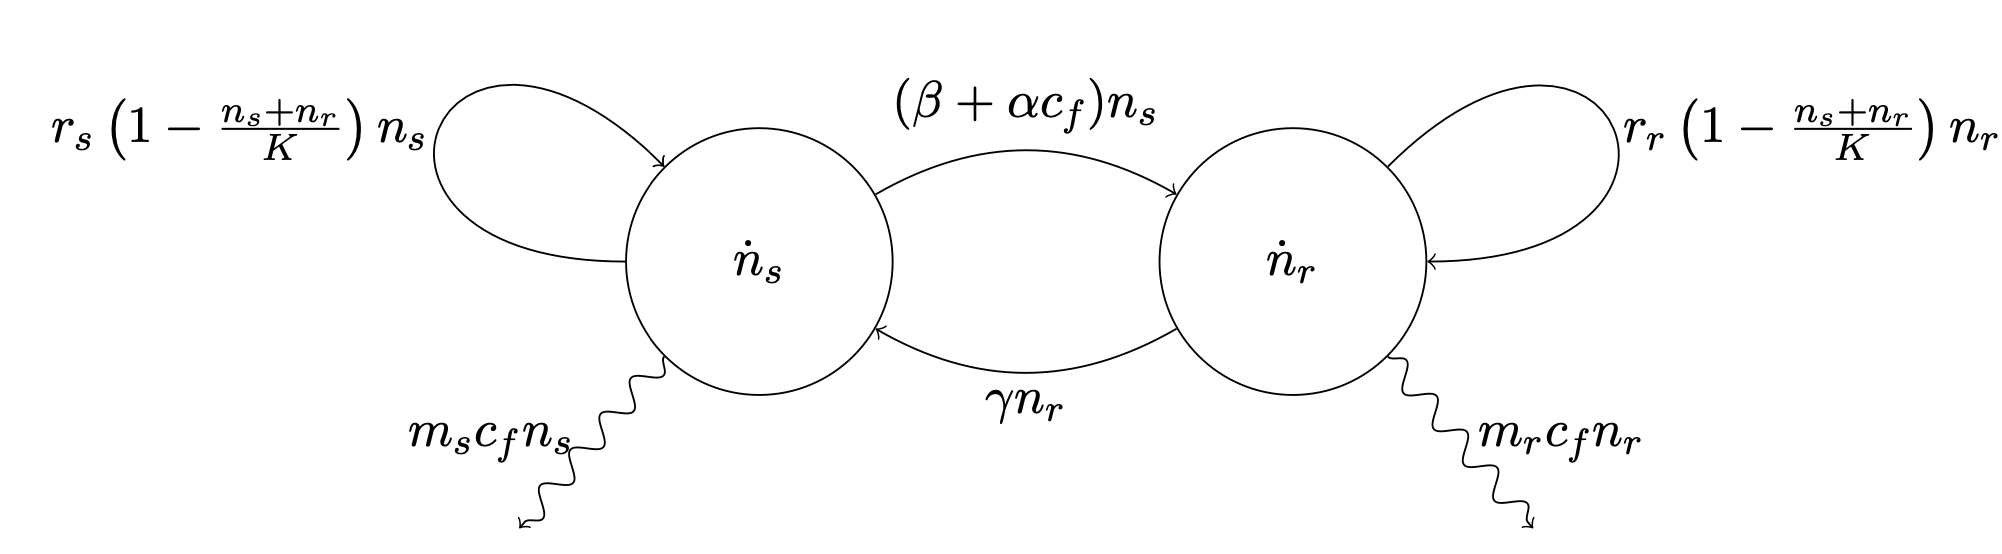
\includegraphics[width=0.7\linewidth]{SchemaModelloCellule.png}
    \caption{Schema del modello~\eqref{eq:system} in cui sono rappresentati i flussi delle cellule.}
    \label{fig:enter-label}
\end{figure}

Si supponga di poter misurare in ogni istante la densità di cellule resistenti $n_r(t)$.


\clearpage
\section{Rappresentazione in Forma di Stato e Linearizzazione del Sistema intorno ad una coppia di equilibrio}

Si riporta il sistema~\eqref{eq:system} nella seguente forma di stato:
%
\begin{subequations}
\begin{align}\label{eq:state_form}
	\dot{x} &= f(x,u)
	\\
	y &= h(x,u).
\end{align}
\end{subequations}
%
Pertanto, si individua lo stato $x$, l'ingresso $u$ e l'uscita $y$ del sistema come segue:
%
\begin{align*}
	x := \begin{bmatrix}
		n_s
		\\
		n_r
	\end{bmatrix}, \quad u := \begin{bmatrix}c_f\end{bmatrix}, \quad y := \begin{bmatrix}n_r\end{bmatrix}.
\end{align*}
%
Coerentemente con questa scelta, si ricava dal sistema~\eqref{eq:system} la seguente espressione per le funzioni $f$ ed $h$:
%
\begin{align*}
	f(x,u) &:=\begin{bmatrix}
		 r_s \bigl(1-\frac{x_1+x_2}{K}\bigr)\, x_1\, -m_s\, u\, x_1\, -\beta\, x_1\, +\gamma\, x_2\, -\alpha\, u\, x_1\ 
	\\
	r_r \bigl(1-\frac{x_1+x_2 }{K}\bigr)\, x_2\, -m_r\, u\, x_2\, +\beta\, x_1\, -\gamma\, x_2\, +\alpha\, u\, x_1\ 
	\end{bmatrix}
\end{align*}
\begin{align*}
	h(x,u) &:= x_2
\end{align*}
%
Una volta calcolate $f$ ed $h$ si esprime~\eqref{eq:system} nella seguente forma di stato:
%
\begin{subequations}\label{eq:our_system_state_form}
\begin{align}
	\begin{bmatrix}
		\dot{x}_1
		\\
		\dot{x}_2
	\end{bmatrix} &= \begin{bmatrix}
	r_s \bigl(1-\frac{x_1+x_2}{K}\bigr)\, x_1\, -m_s\, u\, x_1\, -\beta\, x_1\, +\gamma\, x_2\, -\alpha\, u\, x_1\ 
	\\
	r_r \bigl(1-\frac{x_1+x_2 }{K}\bigr)\, x_2\, -m_r\, u\, x_2\, +\beta\, x_1\, -\gamma\, x_2\, +\alpha\, u\, x_1\ 
\end{bmatrix} \label{eq:state_form_1}
\end{align}
\begin{align}
	y &= x_2
\end{align}
\end{subequations}
%
Per trovare la coppia di equilibrio $(x_e, u_e)$ del punto \eqref{eq:our_system_state_form} si risolve il seguente sistema di equazioni:
%
\begin{align}
	\begin{cases}
		r_s \bigl(1-\frac{n_{s,e}+n_{r,e}}{K}\bigr)\, n_{s,e}\, -m_s\, u_e\, n_{s,e}\, -\beta\, n_{s,e}\, +\gamma\, n_{r,e}\, -\alpha\, u_e\, n_{s,e}\, =0
		\\
		r_r \bigl(1-\frac{n_{s,e}+n_{r,e}}{K}\bigr)\, n_{r,e}\, -m_r\, u_e\, n_{r,e}\, +\beta\, n_{s,e}\, -\gamma\, n_{r,e}\, +\alpha\, u_e\, n_{s,e}\, =0
	\end{cases}
\end{align}
%
dal quale, isolando la $u(t)$, si ottiene:
%
\begin{subequations}
\begin{align}
	u_1(t)=\frac{r_s \bigl(1-\frac{n_{s,e}+n_{r,e}}{K}\bigr)\, n_{s,e}\,-\beta n_{s,e}\,+\gamma n_{r,e}}{(m_s+\alpha)\,n_{s,e}} 
	\\
	u_2(t)=\frac{r_r \bigl(1-\frac{n_{s,e}+n_{r,e}}{K}\bigr)\, n_{r,e}\,+\beta n_{s,e}\,-\gamma n_{r,e}}{m_r\,n_{r,e}+\alpha\,n_{s,e}}
\end{align}
\end{subequations}
%
calcolando quindi rispetto ai parametri forniti si ottiene:
%
\begin{align}
	x_e :=\begin{bmatrix}
		n_{s,e}
		\\
		n_{r,e}
	\end{bmatrix} = 
	\begin{bmatrix}
		100
		\\
		400
	\end{bmatrix},  \quad u_e = 0 \
	\label{eq:equilibirum_pair}
\end{align}
%
Si definiscono le variabili alle variazioni $\delta x$, $\delta u$ e $\delta y$ come:
%
\begin{align*}
	\delta x \approx x(t)-x_e, \\
	\quad 
	\delta u \approx u(t)-u_e, \\
	\quad
	\delta y \approx y(t)-y_e. 
\end{align*}
%
L’evoluzione del sistema, espressa in termini delle variazioni delle variabili, può essere approssimativamente rappresentata attraverso il seguente sistema lineare:
%
\begin{subequations}\label{eq:linearized_system}
\begin{align}
	\delta \dot{x} &= A\delta x + B\delta u
	\\
	\delta y &= C\delta x + D\delta u,
\end{align}
\end{subequations}
%
con opportune matrici $A$, $B$, $C$ e $D$  calcolate nel seguente modo:
%
\begin{subequations}\label{eq:matrices}
\begin{align}
	A &= \begin{bmatrix}
		\frac{\partial}{\partial\,x_1}\,f_1(x,u)\bigg|_{x_e,u_e} & \frac{\partial}{\partial\,x_2}\,f_1(x,u)\bigg|_{x_e,u_e}
		\\
		\frac{\partial}{\partial\,x_1}\,f_2(x,u)\bigg|_{x_e,u_e} & \frac{\partial}{\partial\,x_2}\,f_2(x,u)\bigg|_{x_e,u_e}
	\end{bmatrix} 
	= 
	 \\ &= \begin{bmatrix}
r_s \left(1 - \frac{2x_1 + x_2}{K} \right) - m_s u_e - \beta - \alpha u_e  & -\frac{r_s x_1}{K} + \gamma
		\\
-\frac{r_r x_2}{K} + \beta + \alpha u_e & r_r \left( 1 - \frac{x_1+2x_2}{K} \right) - m_r u_e - \gamma
\end{bmatrix}
	=
	\begin{bmatrix}
		-1.14 & -0.14
		\\
		-0.32 & -1.32
	\end{bmatrix}
	\\ \\ 
	B &= \begin{bmatrix}
		\frac{\partial}{\partial\,u}\,f_1(x,u)\bigg|_{x_e,u_e}
		\\
		\frac{\partial}{\partial\,u}\,f_2(x,u)\bigg|_{x_e,u_e}
	\end{bmatrix}
	=
	\begin{bmatrix}
		-m_s\,x_1-\alpha\,x_1
		\\
		-m_r\,x_2+\alpha\,x_1
	\end{bmatrix}
	=
	\begin{bmatrix}
		-145
		\\
		30
	\end{bmatrix}
	\\ \\
	C &= \begin{bmatrix}
		\frac{\partial}{\partial\,x_1}\,h(x,u)\bigg|_{x_e,u_e} & \frac{\partial}{\partial\,x_2}\,h(x,u)\bigg|_{x_e,u_e}
	\end{bmatrix}
	=\begin{bmatrix}
		0 & 1
	\end{bmatrix}
	\\ \\
	D &= \begin{bmatrix}
		\frac{\partial}{\partial\,u}\,h(x,u)\bigg|_{x_e,u_e}
	\end{bmatrix}
	= \begin{bmatrix}
	0
\end{bmatrix}
\end{align}
\end{subequations}
%
\begin{figure}[h!]
    \centering
    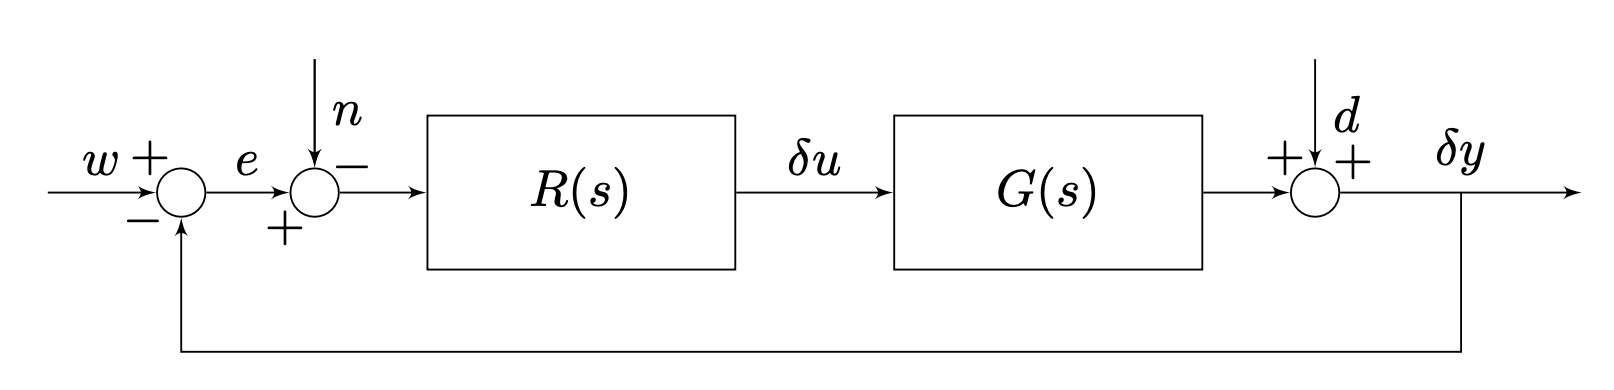
\includegraphics[width=0.7\linewidth]{Figura2.png}
    \caption{Schema di controllo~\eqref{figura2}}
    \label{figura2}
\end{figure}

\clearpage
\section{Calcolo Funzione di Trasferimento}

In questa sezione, si calcola la funzione di trasferimento $G(s)$ dall'ingresso $\delta u$ all'uscita $\delta y$, tale che $\delta Y(s) = G(s)\delta U(s)$,   mediante la seguente formula 
%
%
\begin{align}\label{eq:transfer_function}
G(s) = C(sI-A)^{-1}B-D = 55.2\ \cdot \frac{0.3722s+1}{(s+1)(0.685s+1)}.
\end{align}
%
Dunque il sistema linearizzato~\eqref{eq:linearized_system} è caratterizzato dalla funzione di trasferimento~\eqref{eq:transfer_function} con 2 poli \\ $p_1 = -1.46,  p_2=-1$ e uno zero $z = -2.6867$. In Figura \eqref{bodediagram} si mostra il corrispondente diagramma di Bode. 

\begin{figure}[h!]
    \centering
    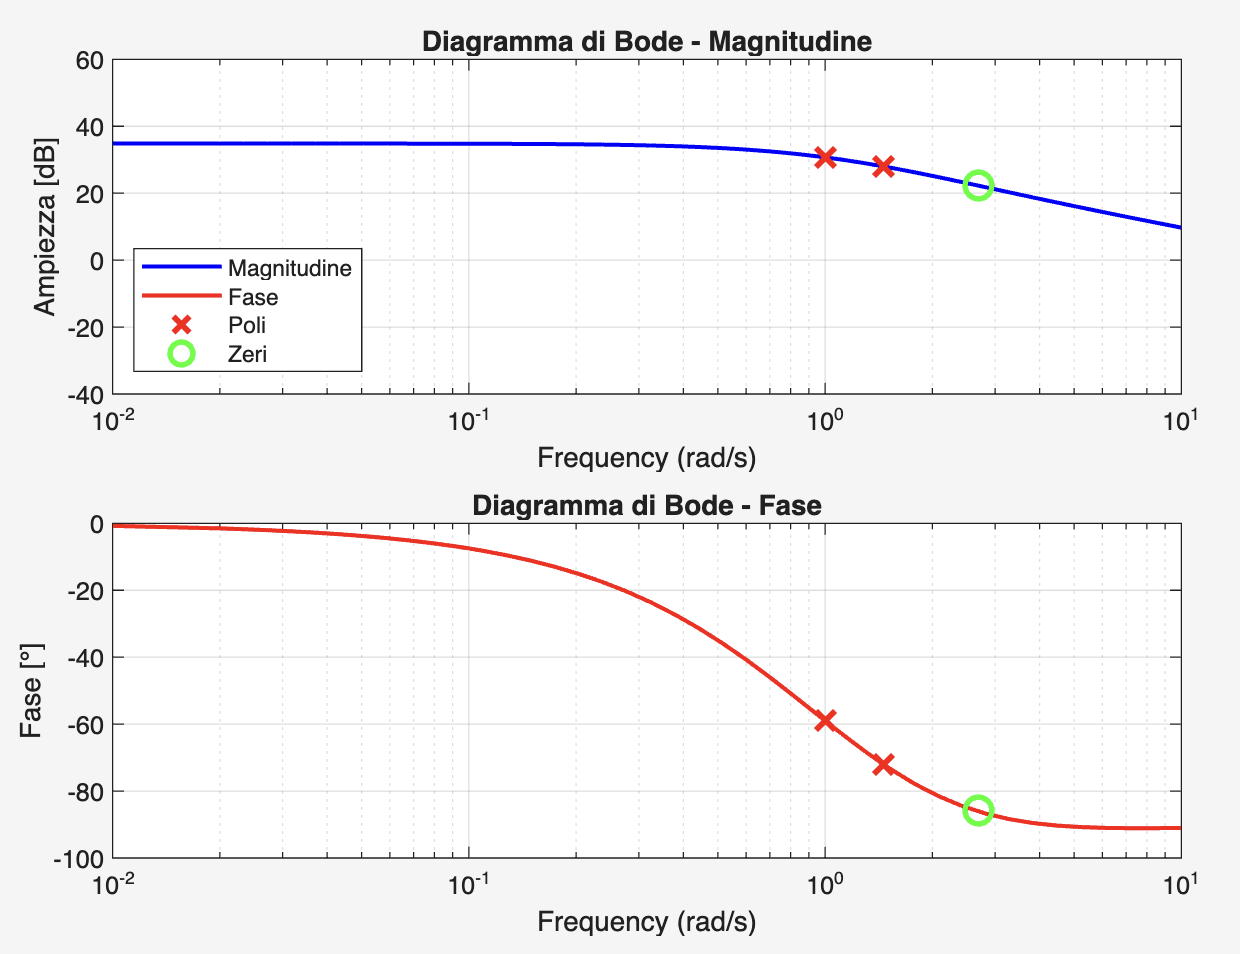
\includegraphics[scale=0.7]{diagramma_bode.png}
    \caption{Diagramma di Bode della funzione di trasferimento G(s)}
    \label{bodediagram}
\end{figure}

\clearpage
\section{Mappatura specifiche del regolatore}
\label{sec:specifications}

Le specifiche da soddisfare sono:
\begin{itemize}
	\item[1)] Errore a regime nullo con:
        \begin{itemize}
    \item riferimento a gradino \( w(t) = -110 \cdot 1(t) \),
    \item disturbo sull'uscita \( d(t) = -20 \cdot 1(t) \)
\end{itemize}
	\item[2)] Per garantire una certa robustezza del sistema si deve avere un margine di fase $M_f\ge45^{\circ}$.\label{spec2}
	\item[3)] La sovraelongazione percentuale massima $S\%\le10\%$\label{spec3}
	\item[4)] Il tempo di assestamento al $\epsilon \% = 5\%$ deve essere inferiore al valore fissato: $T_{\alpha,\epsilon}=0.2s$.\label{spec4}
	\item[5)] Il disturbo in uscita $d(t)$ risulti attenuato di $45dB$ sapendo che la sua banda si limita a pulsazioni nel range $[0;0.1]$\label{spec5}
	\item[6)] Il rumore di misura $n(t)$ con una banda limitata nel range di pulsazioni $[5\cdot10^3;5\cdot10^6]$ deve essera abbattuto di almeno $80dB$ \label{spec6}
\end{itemize}
%
Si procede la mappatura punto per punto delle specifiche richieste. 
\begin{itemize}
	\item[1)] Per azzerare l'errore a regime in risposta ad un segnale a gradino si inserirà un polo nell'origine durante la sintesi del regolatore statico.\
	\item[2)] In corrispondenza della pulsazione critica $\omega_c$ si deve avere una fase maggiore di $-135^{\circ}$\
	\item[3)] Per ottenere una sovraelongazione percentuale massima $S\%\ge10\%$, poniamo $\xi=\frac{M_f}{100}$.
	\\
	Sapendo che la sovraelongazione massima e la $\xi$ massima rispettano la seguente relazione:\\
	 $S^\star=e^\frac{-\pi\xi^\star}{\sqrt{1-(\xi^\star)^2}}$. e quindi: \\
     \[
        \xi^* = \left| \frac{\ln{\left(\frac{S^*}{100}\right)}}{\sqrt{\pi^2 + \ln^2{\left(\frac{S^*}{100}\right)}}} \right|
        \]
        
        \[
        M_{f,S^*} = 100 \cdot \xi^*
        \]
	 \\
	 Sostituendo $\xi$ otteniamo $M_f\ge59,1^{\circ}$.
	\item[4)] Per ottenere un tempo di assestamento al $5\%$ inferiore al valore fissato  $T_{a,\epsilon}=0.2s$ è necessario imporre $e^{-\xi\omega_c\,T_a}=0.05$.\\
	Si ottiene quindi $\xi\omega_c\ge\frac{3}{T^\star}$ con $T^\star$ tempo di assestamento massimo.\\
	Da ciò si ricava quindi $\omega_c=\frac{300}{T^\star\,M_f}=25.374\frac{rad}{s}$.
	\item[5)] Per riuscire ad attenuare il disturbo in uscita $d(t)$ di 45dB risulta necessario che nell'intervallo d'interesse($[0;0.1]$) $|L(j\omega)|_{dB}\ge45dB$.\
	\item[6)] Per riuscire ad attenuare il disturbo di misura $n(t)$ di 80dB risulta necessario che nell'intervallo d'interesse($[5\cdot10^3;5\cdot10^6]$) $|L(j\omega)|_{dB}\le-80dB$.\
\end{itemize}
\clearpage
Pertanto, in Figura \ref{bodepatch}, si mostra il diagramma di Bode della funzione di trasferimento $G(s)$ con le zone proibite emerse dalla mappatura delle specifiche.

\begin{figure}[h!]
    \centering
    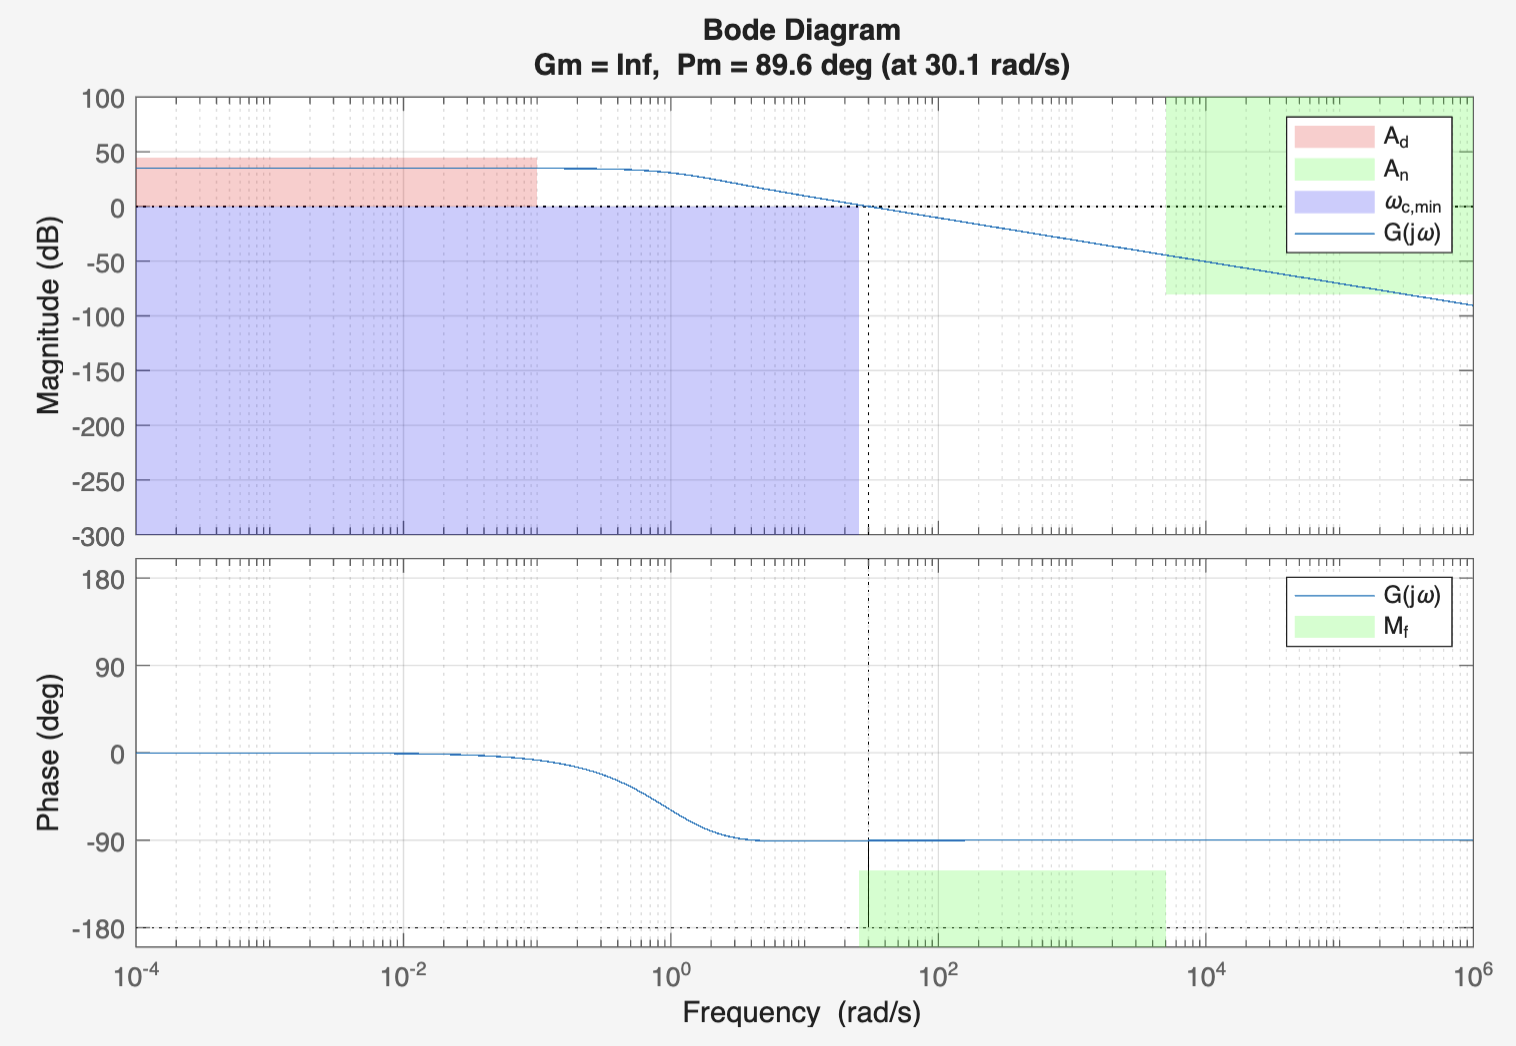
\includegraphics[width=1\linewidth]{bode_patch.png}
    \caption{Diagramma di Bode di G(s) con patch delle zone proibite}
	\label{bodepatch}
\end{figure}

\clearpage
\section{Sintesi del regolatore statico}
\label{sec:static_regulator}


In questa sezione si progetta il regolatore statico $R_s(s)$ partendo dalle analisi fatte in sezione~\ref{sec:specifications}.\\
La progettazione del regolatore statico è volta alla risoluzione delle problematiche dovute alle specifiche $1$ e $5$ viste nel punto precedente.\\
Per ottenere errore a regime nullo in risposta al riferimento a gradino, inseriamo un polo nell'origine. 
Abbiamo calcolato $\mu_s$ come:
\begin{equation}
    \mu_s = \frac{10^{\frac{A_d}{20}}}{G(j\omega_{d,\text{max}})} =  3.243 \cdot 10^{-1}
\end{equation}

per ottenere l'attenuazione richiesta di $45dB$ sul disturbo in uscita $d(t)$ a basse pulsazioni.
\\
\\
Il regolatore statico così sintetizzato risulta essere nella forma $R_s(s)=\frac{\mu_s}{s}$.\\

Dunque, si definisce la funzione estesa $G_e(s) = R_s(s)G(s)$ e, in Figura \ref{geconpatch}, mostrando il suo diagramma di Bode per verificare se e quali zone proibite vengono attraversate.

\begin{figure}[h!]
    \centering
    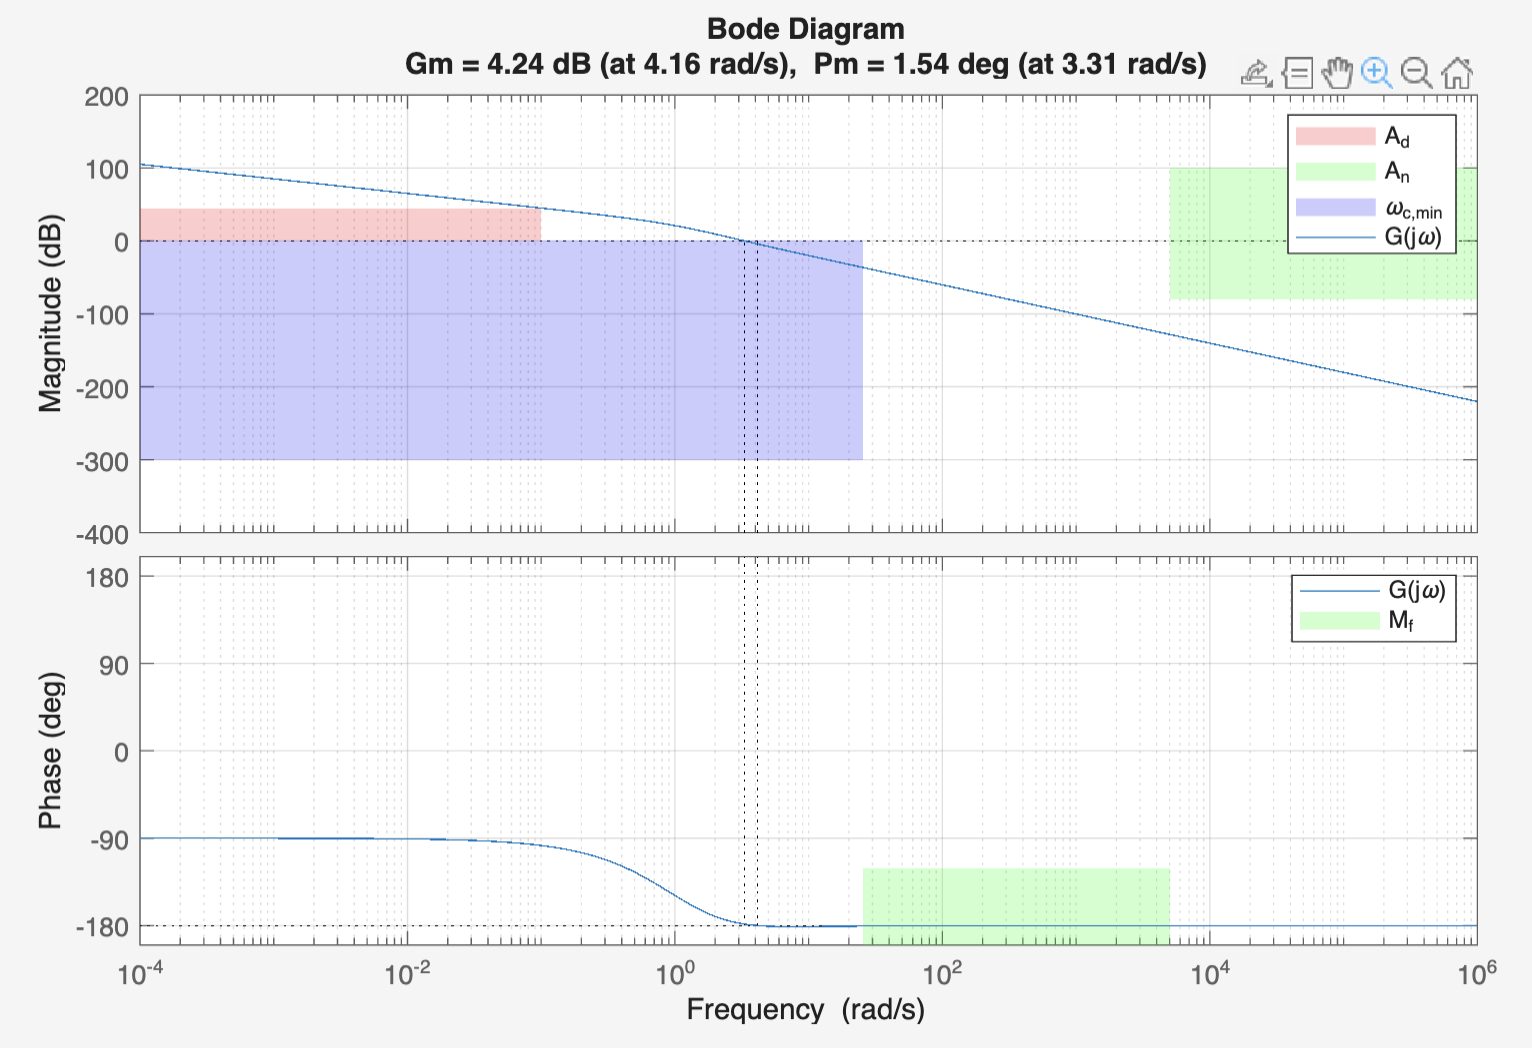
\includegraphics[width=0.6\linewidth]{GeConPatch.png}
    \caption{Diagramma di Bode del sistema esteso con patch delle zone proibite}
    \label{geconpatch}
\end{figure}


Da Figura \ref{geconpatch} si può osservare che le specifiche riguardanti il disturbo di uscita $d(t)$ e quello di misura $n(t)$ risultano rispettate dato che $|L(j\omega)|_{dB}\ge45dB$ a basse frequenze e $|L(j\omega)|_{dB}\le-80dB$ ad alte frequenze. \\
La specifica sul margine di fase risulta essere rispettata, dato che in prossimità dell'attraversamento degli $0$ $dB$ nel diagramma delle ampiezze, in quello della fase ci si trova fuori dalla patch verde. \\
Non risulta essere rispettato il vincolo sulla $\omega_{c,min}$, espresso dalla patch blu. Questa problematica verrà risolta con la sintesi del regolatore dinamico. \\
La fase del sistema esteso, non supera i $-180^{\circ}$. Ciò rispetta il teorema di Bode, il cui enunciato dice che, rispettate le ipotesi riguardo l'attraversamento dello 0 in un solo punto e la mancanza di poli a parte reale positiva (ipotesi rispettate dal nostro sistema), condizione necessaria e sufficiente per la stabilità di un sistema retroazionato è che la sua $L(j\omega)$ (in questo caso la nostra $G_e(s)$) risulti avere fase maggiore di $-180^{\circ}$ alla pulsazione critica $\omega_c$. \\


\clearpage
\section{Sintesi del regolatore dinamico}

In questa sezione, si progetta il regolatore dinamico $R_d(s)$. \\
%
Dalle analisi fatte in Sezione~\ref{sec:static_regulator}, si e' osservato che il sistema si trova nello Scenario di tipo B, in cui tutto l'intervallo d'interesse per la nostra $\omega_c$ risulta avere fase minore di $-120.9^{\circ}$($-180^{\circ}+M_f$). \\
Dunque, progettiamo $R_d(s)$ inserendo una rete anticipatrice, essendoci il bisogno di alzare il diagramma di fase
di almeno $40^{\circ}$. 



Procediamo dunque alla progettazione del regolatore dinamico $R_d(s)$.
\\
Una rete anticipatrice è della forma:
\[
R_{ant}(s) = \frac{1 + \tau s}{1 + \alpha \tau s}
\]

Calcoliamo i valori di \( M^* \) e \( \varphi^* \):
\[
M^* = \frac{1}{\lvert G_e(j\omega_c^*) \rvert} \approx 92.3
\]
\[
\varphi^* = (M_{f,S^*} + 5^\circ) - 180^\circ - \arg(G_e(j\omega_c^*)) \approx -295.5^\circ
\]

Il valore di $\varphi^*$ diventa $64.5^\circ$ (convertito in un valore positivo aggiungendo $360^\circ)$. \\
Il valore di \( M_{f,S^*} \) è stato aumentato di \( 5^\circ \) per essere conservativi. Avendo \( M^* > 1 \) e \( 0 < \varphi^* < \frac{\pi}{2} \) come richiesto dalla specifica della rete anticipatrice, calcoliamo i valori di \( \tau \) e \( \alpha \tau \):
\[
\tau = \frac{M^* - \cos\varphi^*}{\omega_c^* \sin\varphi^*} \approx 3.3921
\]
\[
\alpha \tau = \frac{\cos\varphi^* - \frac{1}{M^*}}{\omega_c^* \sin\varphi^*} = 1.55 \cdot 10^{-2} 
\]

Dopo la sintetizzazione del regolatore dinamico il sistema risulta essere correttamente regolato. \\
In Figura \ref{bodepostdinamic}, mostriamo il diagramma di Bode della funzione d'anello $L(s) = R_d(s) G_e(s)$


\begin{figure}[h!]
    \centering
    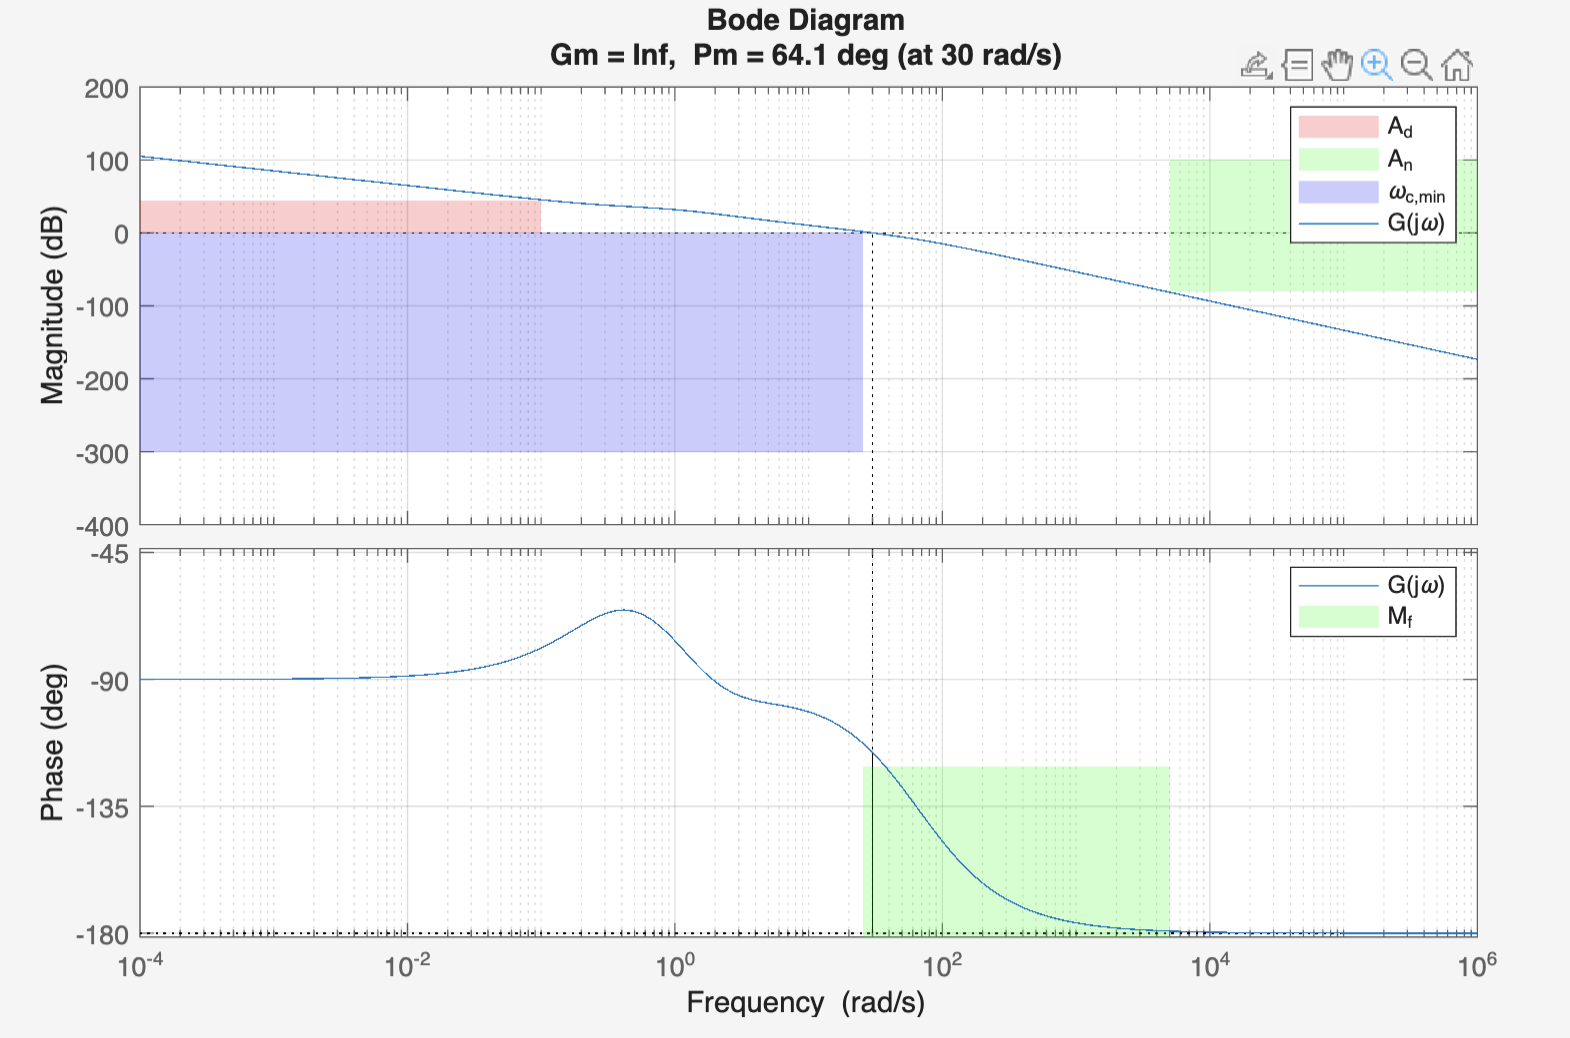
\includegraphics[width=0.8\linewidth]{Bode_post_r_dinamico.png}
    \caption{Diagramma di Bode del sistema esteso con regolatore dinamico completo.}
    \label{bodepostdinamic}
\end{figure}


\clearpage
\section{Test sul sistema linearizzato}
\label{sec:testsistemalinearizzato}

In questa sezione, si testa l'efficacia del controllore progettato sul sistema linearizzato in risposta a segnali:
\begin{align*}
w(t) &= -110 \cdot 1(t) \\
d(t) &= \sum_{k=1}^{4} -2 \cdot \sin(0.025k t) \\
n(t) &= \sum_{k=1}^{4} 0.1 \cdot \sin(5\cdot10^3k t)
\end{align*}
\\
Dopo aver ricavato le funzioni di sensitività $F(s)$ e $S(s)$ si analizza la risposta del sistema al segnale a gradino $w(t)$ (in Figura \ref{Figura 6}), al disturbo $d(t)$ (in Figura \ref{Figura 7}) e al disturbo $n(t)$ (in Figura \ref{Figura 8}).

Le funzioni di sensitività si calcolano come segue:
\[
    F(s) = \frac{L(s)}{1 + L(s)} 
    \]
    \[
    S(s) = \frac{1}{1 + L(s)}
\]

Dove \( L(s) \) rappresenta la funzione d'anello del sistema. 

\\
\begin{figure}[H]
	\centering
	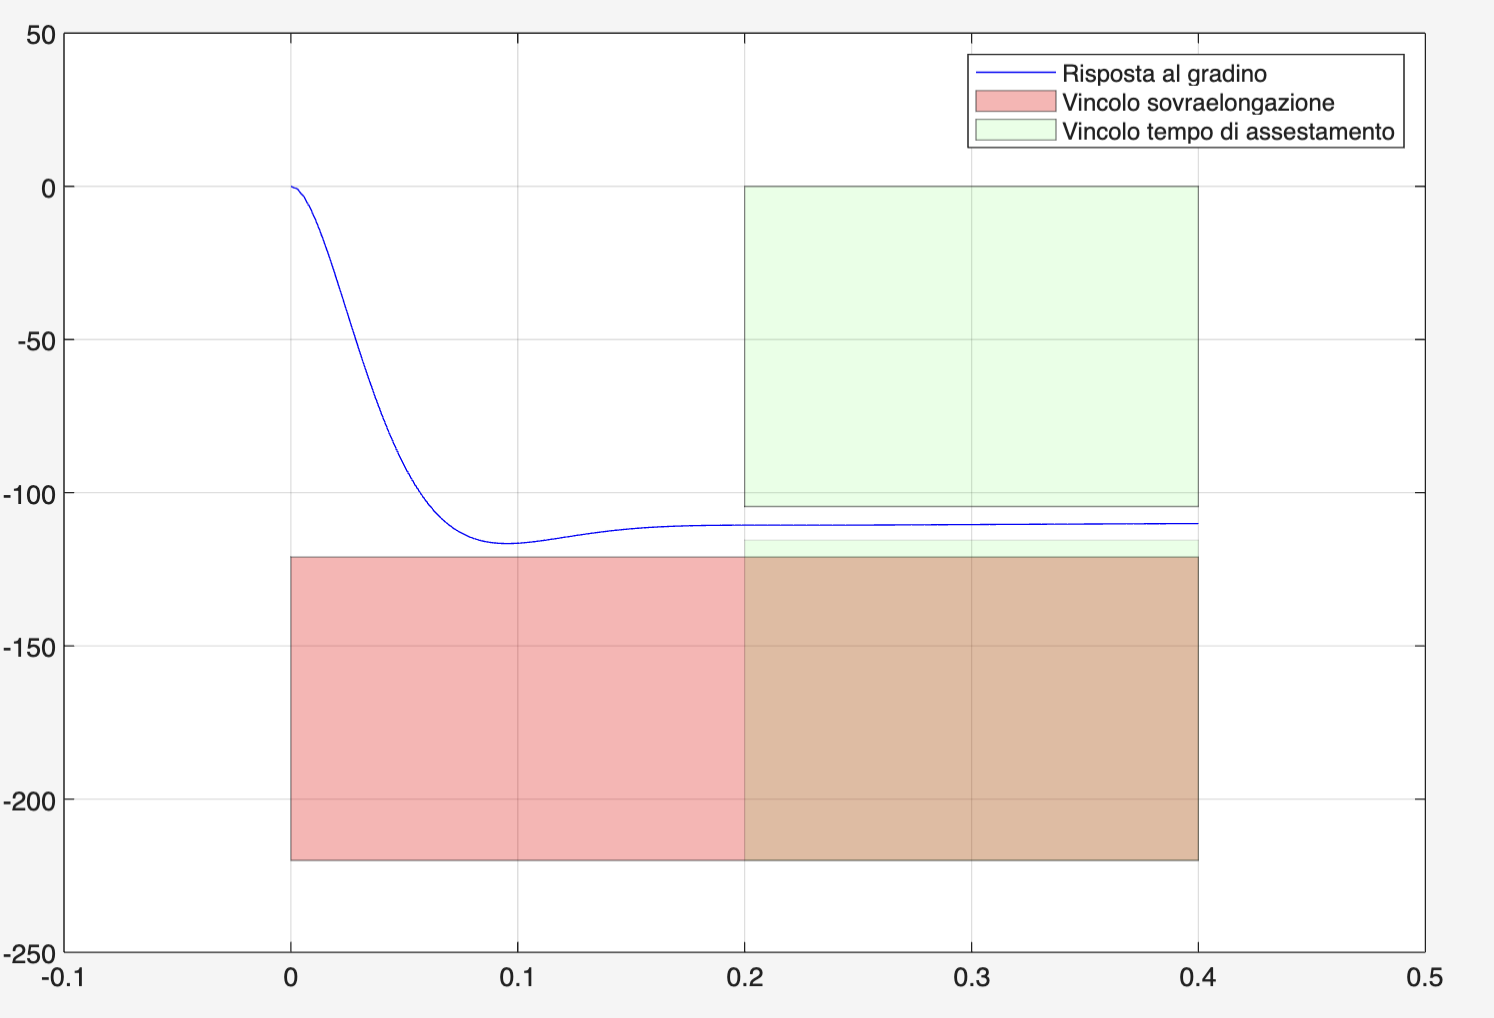
\includegraphics[width=12cm]{Risposta_gradino.png}
	\caption[]{Risposta al gradino con vincoli di sovraelongazione e tempo di assestamento evidenziati}
	\label{Figura 6}
\end{figure}
\begin{figure}[H]
	\centering
	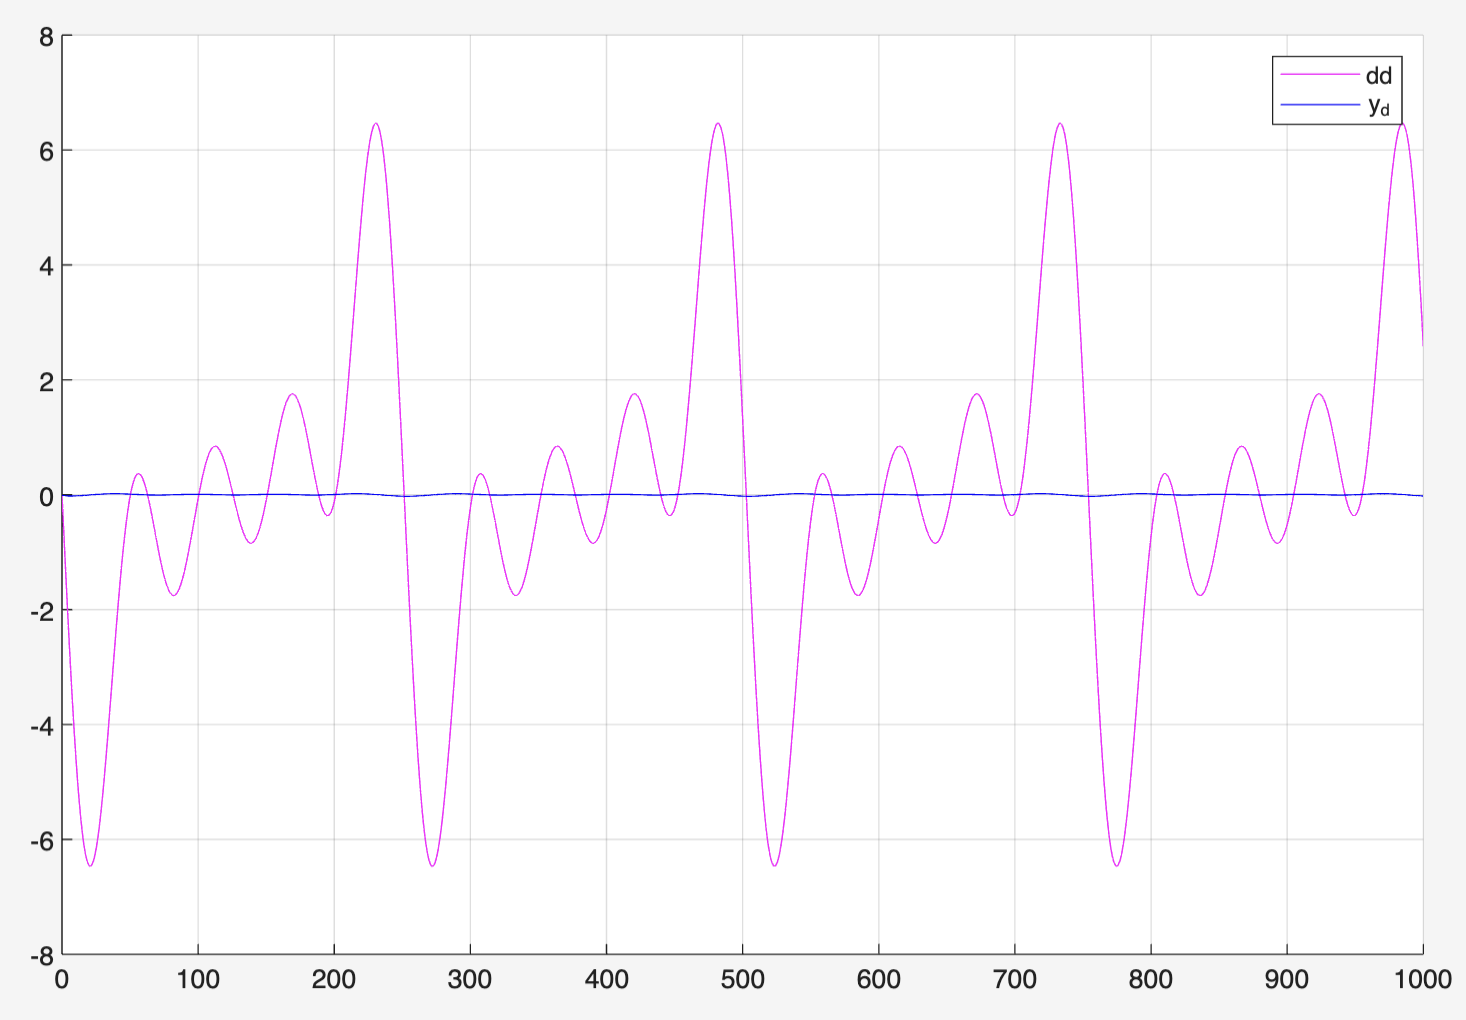
\includegraphics[width=12cm]{Risposta_dd.png}
	\caption[]{Risposta al disturbo $d(t)$}
	\label{Figura 7}
\end{figure}

\begin{figure}[H]
	\centering
	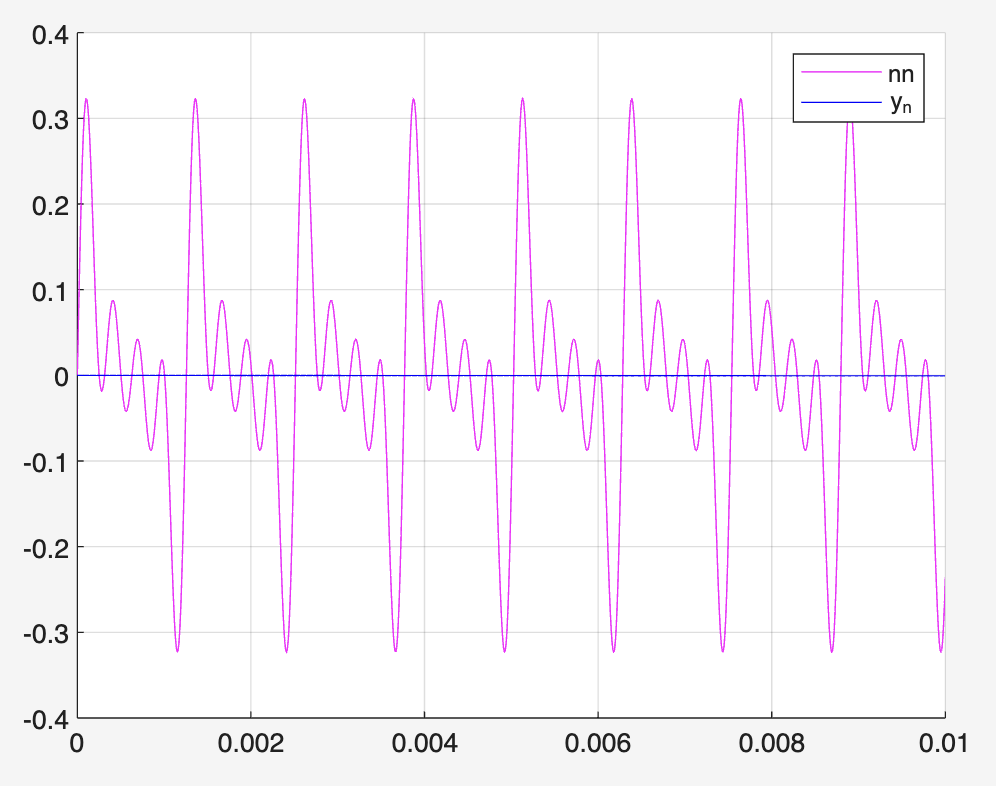
\includegraphics[width=12cm]{Risposta_nn.png}
	\caption[]{Risposta al disturbo $n(t)$}
	\label{Figura 8}
\end{figure}

Si osserva che $y_w(t)$ rispetta pienamente le specifiche, inoltre $y_d(t)$ e $y_n(t)$ risultano essere attenuati in accordo ai requisiti.
\\
\clearpage

Si procede ora a sommare le tre risposte per ottenere il grafico della risposta complessiva del sistema (In Figura ee\ref{Figura 9}).\\
\begin{figure}[H]
    \centering
    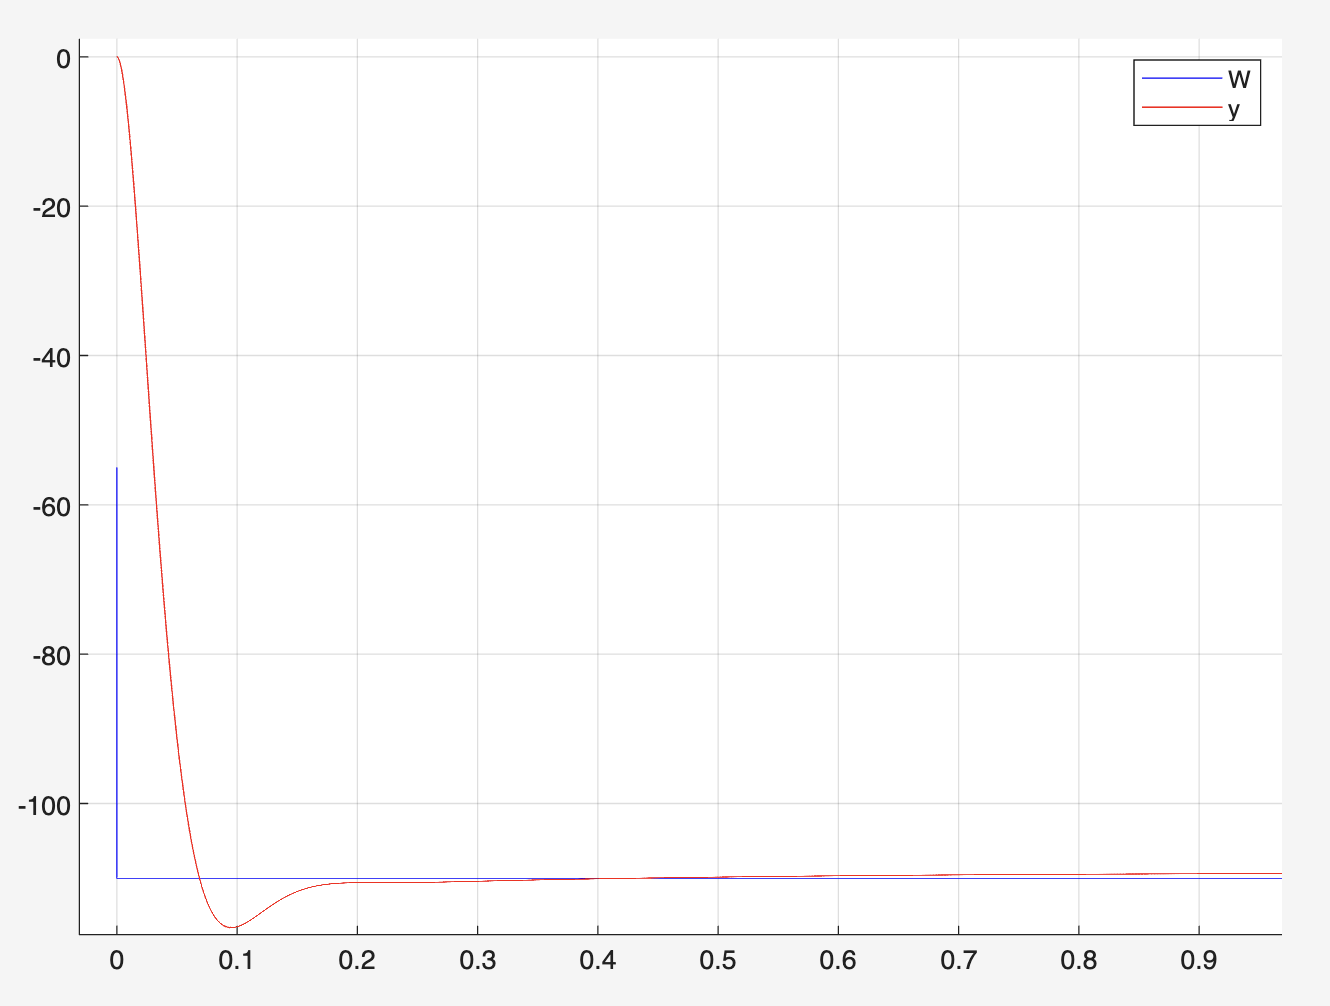
\includegraphics[width=12cm]{Risposta_complessiva.png}
    \caption[]{Risposta complessiva $y(t)$}
    \label{Figura 9}
\end{figure}

\clearpage
\section{Test sul sistema non lineare}

In questa sezione si testa l'efficacia del controllore progettato sul modello non lineare in riferimento ai segnali visti nella Sezione \ref{sec:testsistemalinearizzato}.
\\
Per effettuare i test si è utilizzato l'ambiente Simulink offerto da Matlab.
Si è realizzato un modello di sistema in retroazione così strutturato.
\begin{figure}[H]
	\centering
	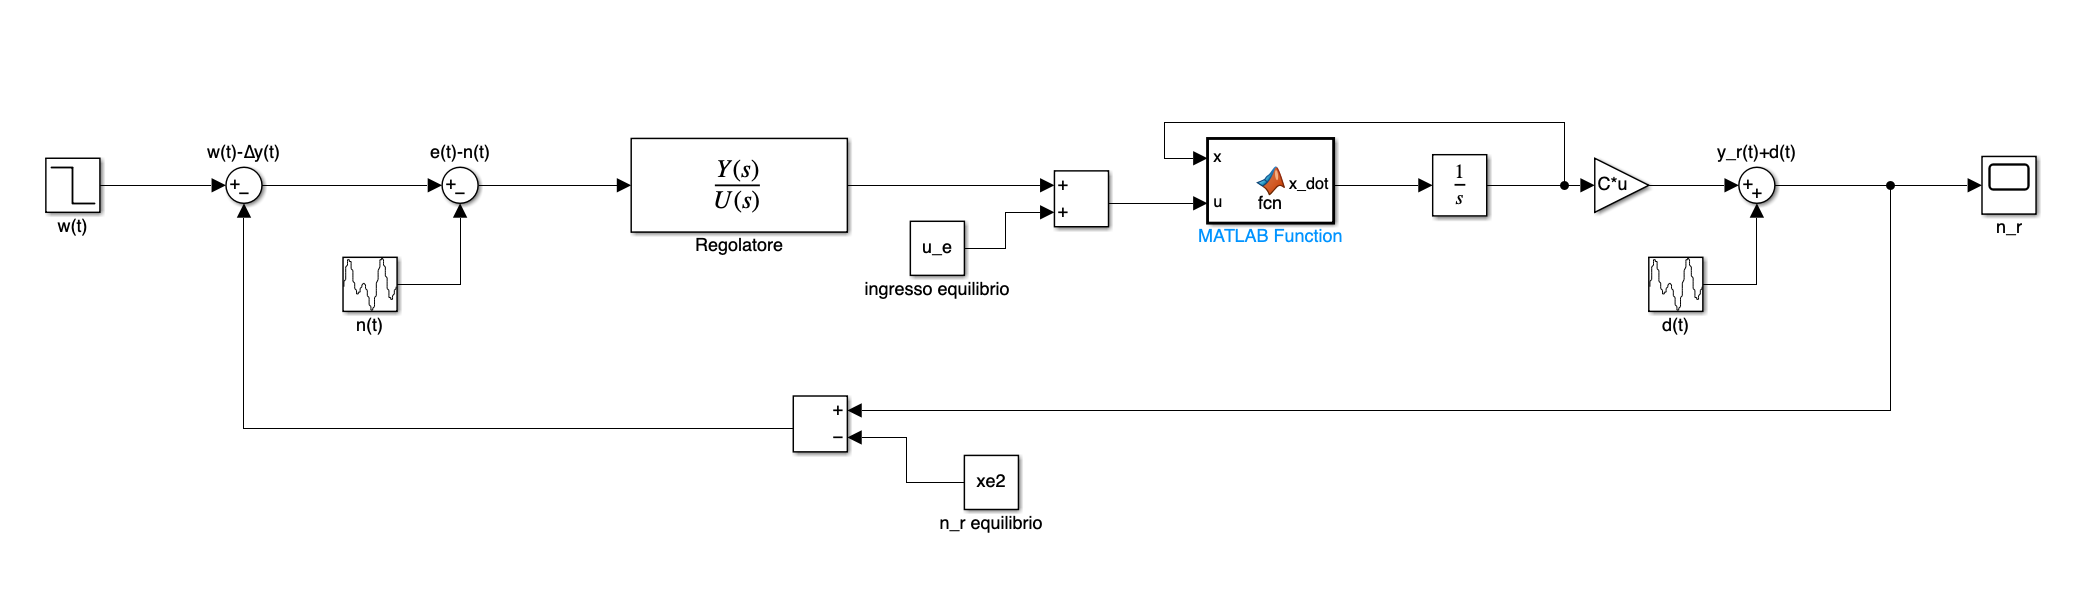
\includegraphics[width=1\linewidth]{SistemaNonLineare.png}
	\caption[]{Sistema non linearizzato}
	\label{Figura 11}
\end{figure}

Nel blocco della funzione sono stati riportati i dati del sistema non linearizzato, rappresentati in figura \ref{datibloccononlineare}
\begin{figure}[h!]
	\centering
	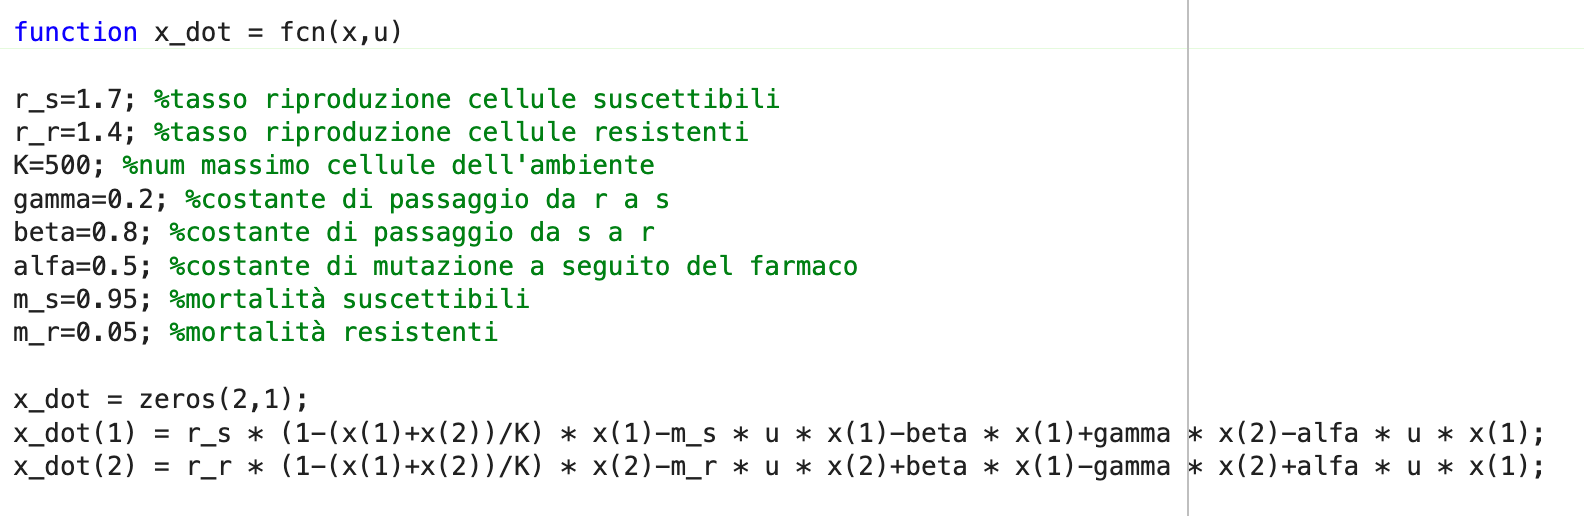
\includegraphics[width=0.9\linewidth]{Dati_blocco_non_lineare.png}
	\caption[]{Dati del sistema non linearizzato}
	\label{datibloccononlineare}
\end{figure}

Nel caso di test riportato vengono considerate condizioni iniziali $x_0=\begin{bmatrix}
	100
	\\
	400
\end{bmatrix}$, il cui risultato è visibile in Figura \ref{Figura 13}
\begin{figure}[H]
	\centering
	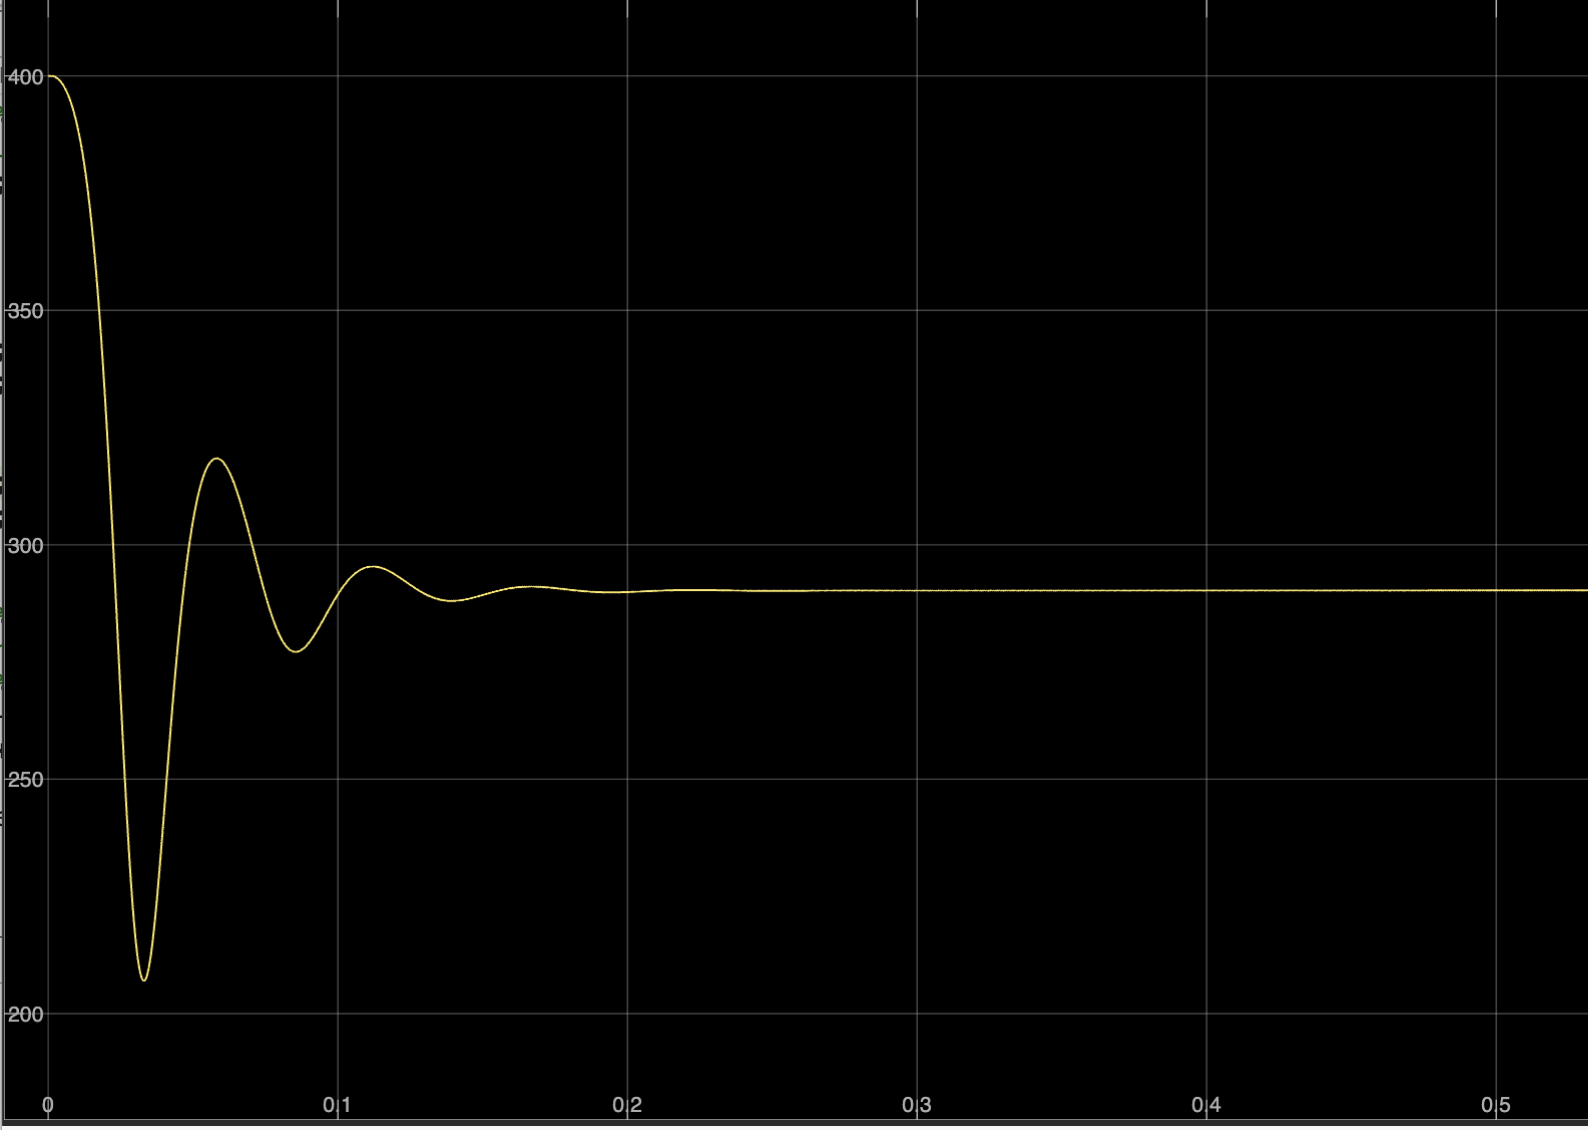
\includegraphics[width=12cm]{TestSistemaNonLinearizzato.png}
	\caption[]{Test del regolatore sul sistema non lineare}
	\label{Figura 13}
\end{figure}

A seguito dei test effettuati il sistema risulta essere stabile e regolato, poichè in accordo con le specifiche fornite.

\clearpage
\section{Punti opzionali}
\subsection{Primo punto}
Per visualizzare l'evoluzione della densità di cellule all'interno della coltura si è scelto di utilizzare sia un diagramma a barre (\ref{Figura 14}) per una visualizzazione statica, che un grafico con slider(\ref{Figura 15}) per un'animazione più dinamica.
\begin{figure}[H]
	\centering
	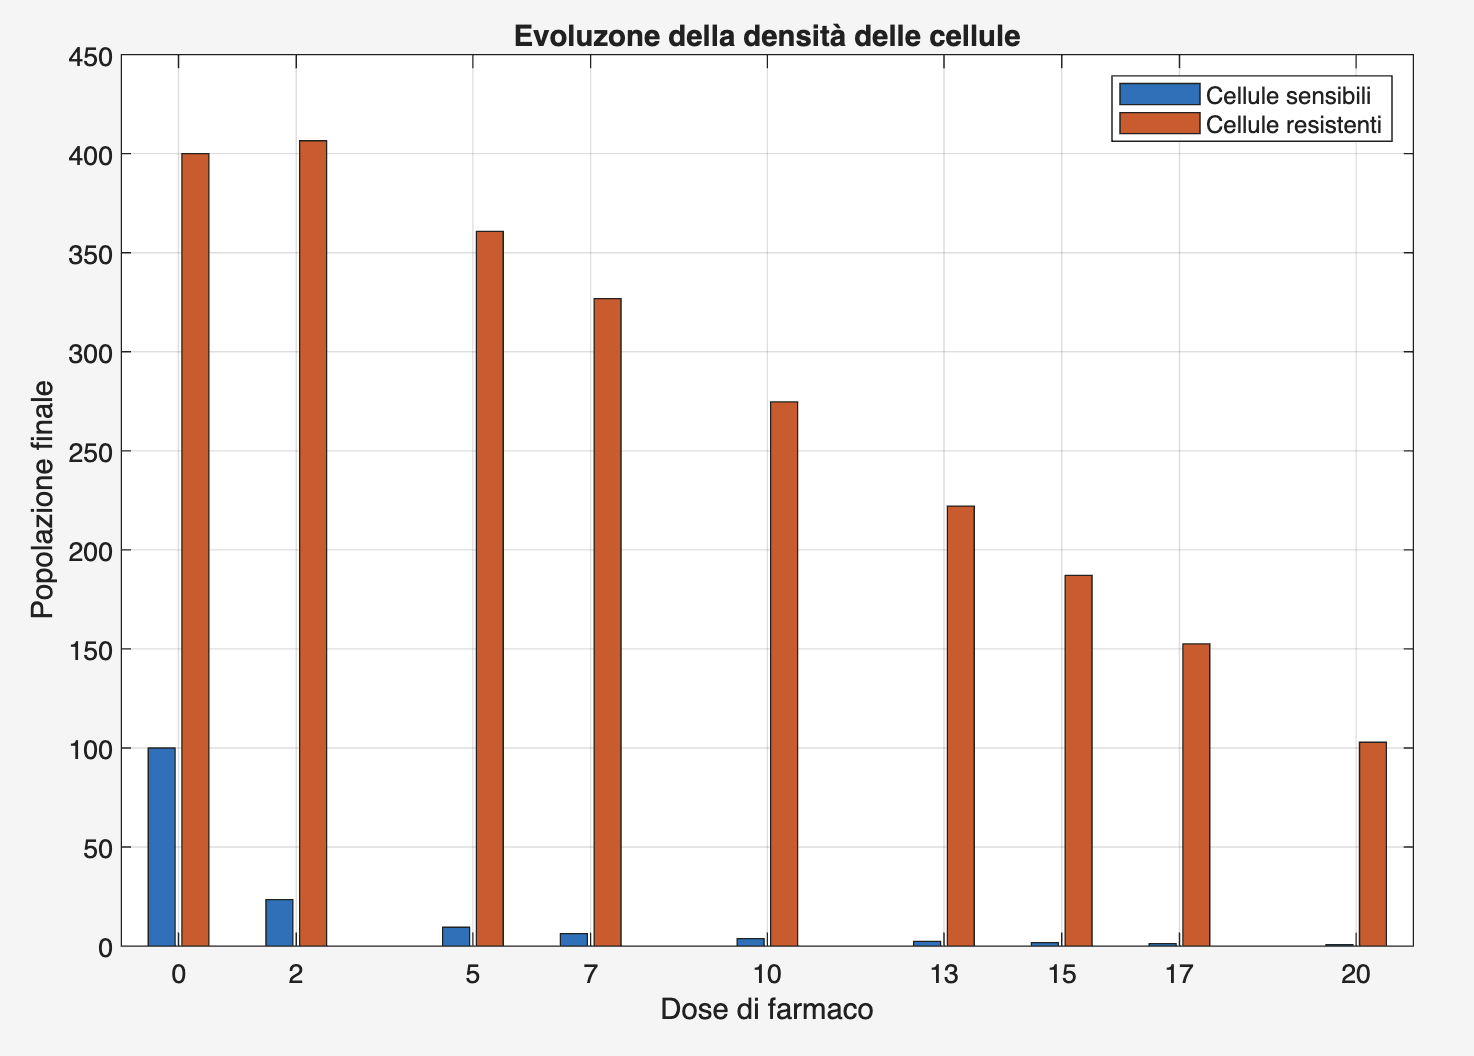
\includegraphics[width=12cm]{Primopuntoopzionale_1.png}
	\caption[]{Evoluzione della densità di cellule: diagramma a barre}
	\label{Figura 14}
\end{figure}
\begin{figure}[H]
	\centering
	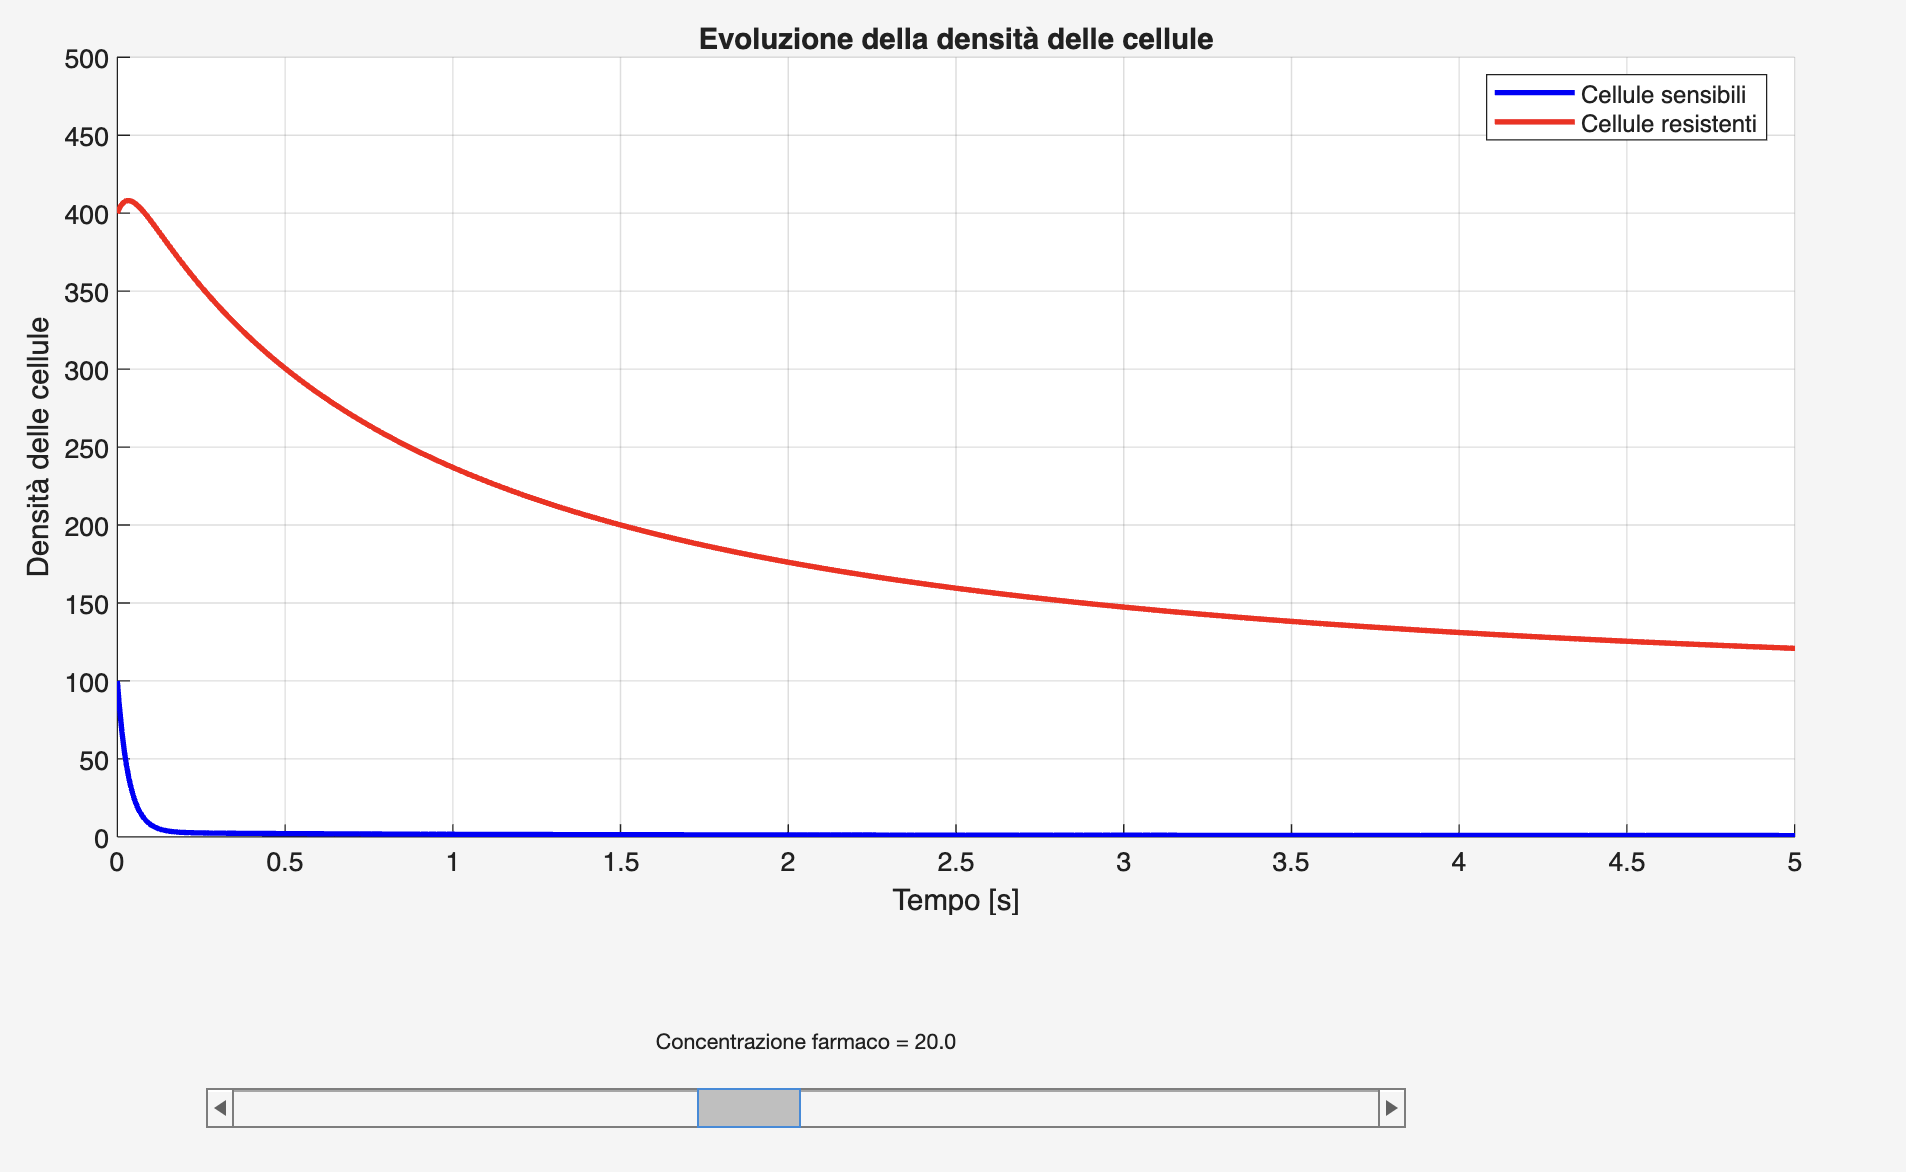
\includegraphics[width=12cm]{Primopuntoopzionale_2.png}
	\caption[]{Evoluzione della densità di cellule: grafico con slider}
	\label{Figura 15}
\end{figure}

\clearpage
\subsection{Secondo punto}
In questo punto si analizza il range di condizioni iniziali (nell’intorno del punto di equilibrio) tali per cui l’uscita del sistema in anello chiuso converga a $h(x_e,u_e)$, corrispondente alla variabile $x_2$. Variando $x_1$ e mantenendo $x_2$ costante $(x_2=x_{2,e})$ si osserva da Figura \ref{Figura 16} che l’uscita converge al punto di equilibrio rispettando le specifiche del sistema. Il range di valori per x1 corrisponde a quelli fisicamente validi, ossia maggiori di 0, in quanto la densità non può essere negativa. 
\\
 \begin{figure}[H]
 	\centering
 	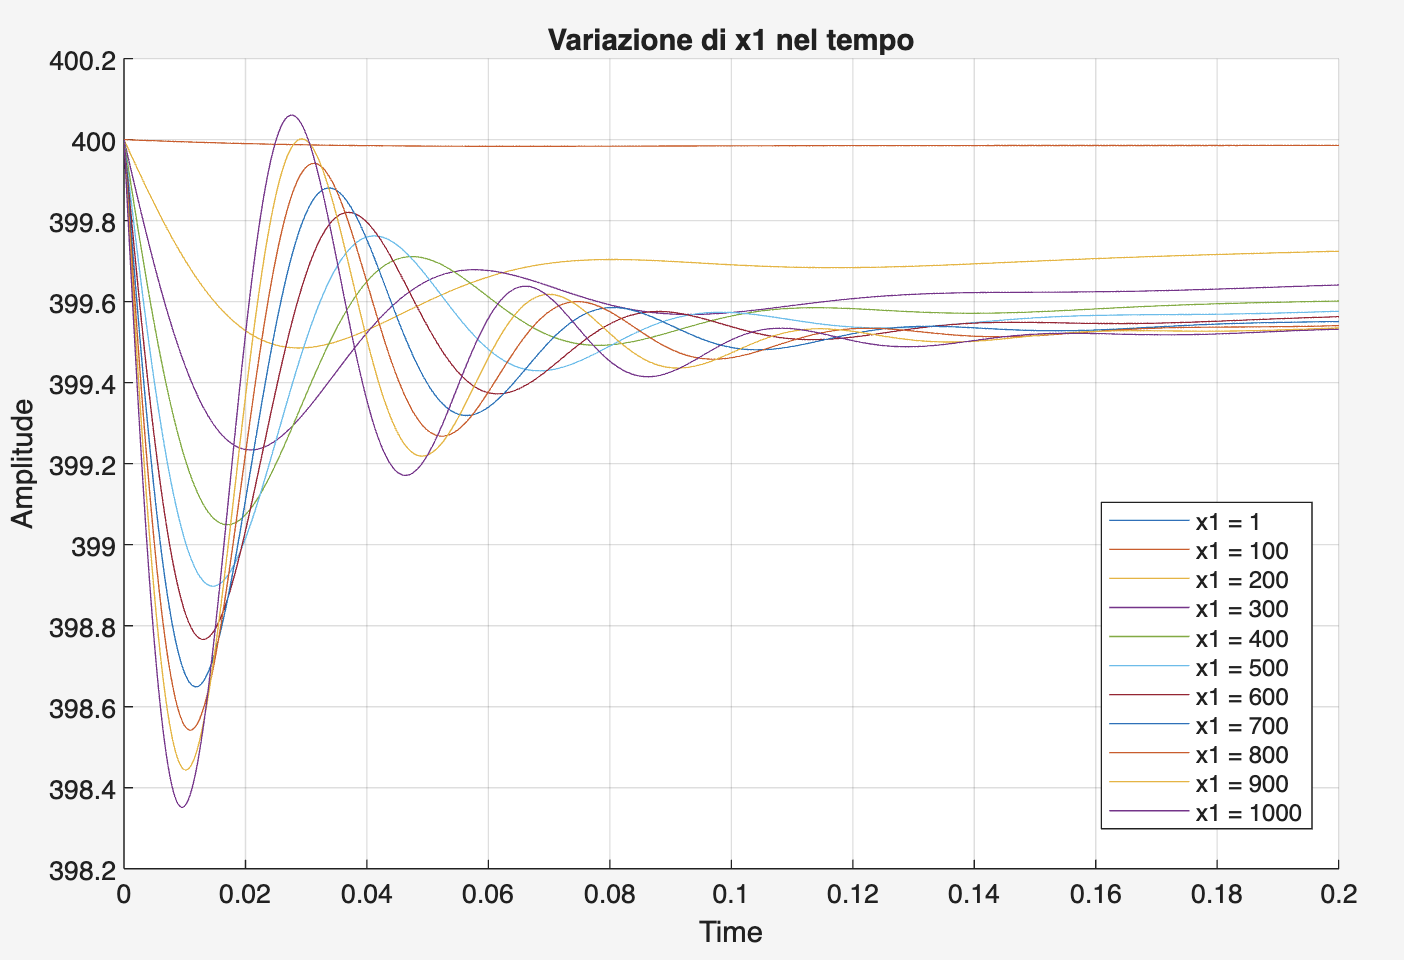
\includegraphics[width=0.6\linewidth]{Secondopuntoopzionale_1.png}
 	\caption[]{Range di variazioni di $x_1$}
 	\label{Figura 16}
 \end{figure}
 Procedimento analogo per la variazione di $x_2$, in cui abbiamo notato che la convergenza avviene con un massimo più elevato rispetto a quello riportato in figura. Per semplicità, tuttavia, limitiamo la rappresentazione grafica ai valori mostrati. Il valore minimo, invece, è stato approssimato considerando che, al di sotto di esso, il vincolo sul tempo di assestamento non risulta rispettato. Infatti, a  $t=0.2s$ , la funzione non rientra nel range del 5\% [380, 420].
\begin{figure}[H]
    \centering
    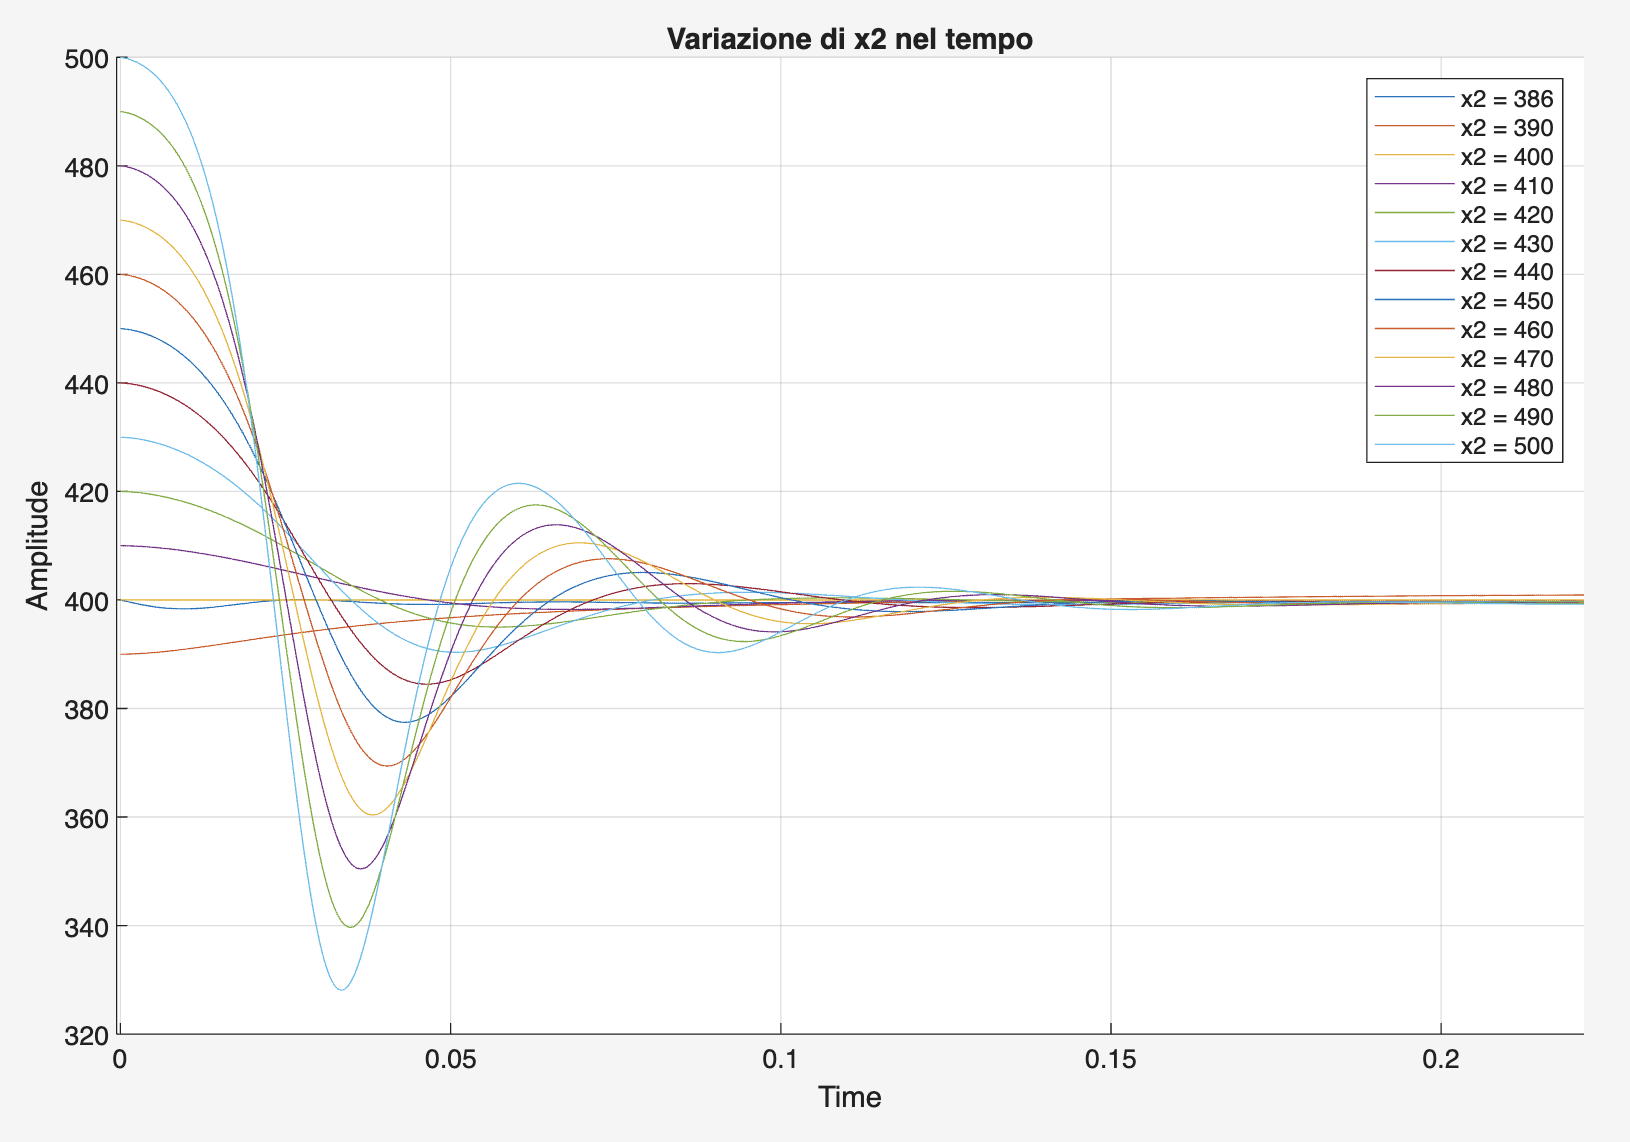
\includegraphics[width=0.6\linewidth]{Secondopuntoopzionale_2.png}
    \caption[]{Range di variazioni di $x_2$}
    \label{Figura 17}
\end{figure}


\subsection{Terzo punto}
In questo punto si analizza il range di ampiezza di riferimenti a gradino tali per cui il controllore rimane efficace sul sistema non lineare.
Vediamo in Figura \ref{Figura 18} che variando l’ampiezza di $w(t)$ in un range [-1110,1000] il controllore rimane efficace. In particolare si nota che i vincoli del sistema sono soddisfatti poichè in prossimità di $T_{a,\epsilon}$ la funzione rientra nel range del 5\% .
\\

\begin{figure}[H]
	\centering
	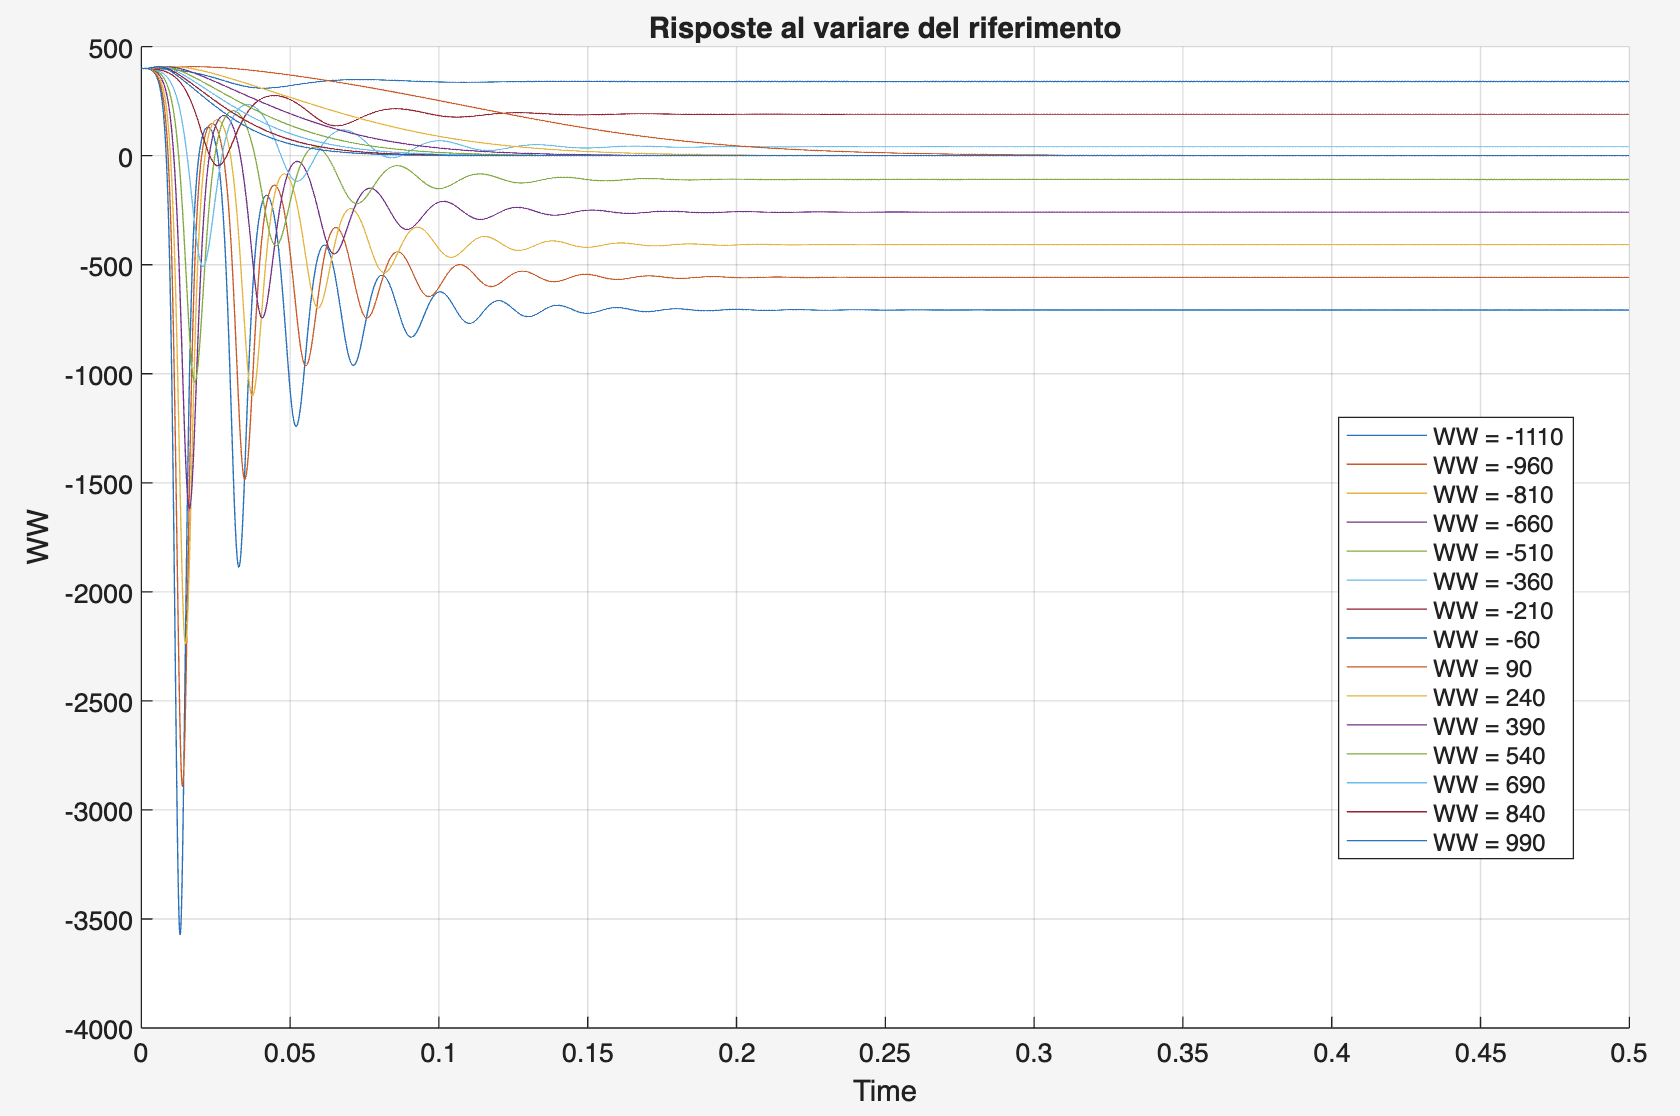
\includegraphics[width=0.8\linewidth]{Terzopuntoopzionale.png}
	\caption[]{Variazione dell'ampiezza di $w(t)$}
	\label{Figura 18}
\end{figure}
\section{Conclusioni}


Il progetto mira a realizzare un regolatore che permette il trattamento farmacologico di cellule in ambiente di laboratorio.
\\
Inizialmente, il sistema è stato linearizzato attorno al punto di equilibrio per facilitare l’analisi e la progettazione. 
A partire da questa linearizzazione, abbiamo sviluppato un regolatore, composto da un parte statica $R_s$ e una dinamica $R_d$, con l’obiettivo di soddisfare le specifiche di errore a regime, ridurre l’attenuazione del disturbo sia in uscita che in misura, e controllare la sovraelongazione massima e il tempo di assestamento.
\\
Completata la progettazione, abbiamo testato il comportamento del sistema linearizzato, eseguendo simulazioni che includessero disturbi sia in uscita che in misura. Analizzando in modo approfondito il sistema in anello chiuso, tramite queste simulazioni, si nota la sua capacità di mantenere il rispetto delle specifiche progettuali e di rispondere in modo adeguato ai disturbi applicati.
\\
Successivamente, ci siamo occupati del sistema non lineare, eseguendo simulazioni con gli stessi disturbi che erano stati impiegati nel contesto linearizzato. 
Questo confronto ci ha permesso di osservare le differenze tra il comportamento del sistema linearizzato e quello non linearizzato, mettendo in risalto la sua capacità di gestire i disturbi, evidenziando le  performance e le potenzialità del regolatore progettato in uno scenario reale.

\clearpage
\begin{figure}
    \centering
    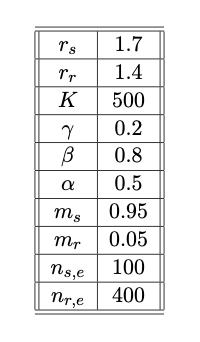
\includegraphics[width=0.2\linewidth]{tabella_parametri}
    \caption{Tabella parametri}
    \label{fig:enter-label}
\end{figure}

\end{document}

